\documentclass[12pt,]{book}
\usepackage{lmodern}
\usepackage{amssymb,amsmath}
\usepackage{ifxetex,ifluatex}
\usepackage{fixltx2e} % provides \textsubscript
\ifnum 0\ifxetex 1\fi\ifluatex 1\fi=0 % if pdftex
  \usepackage[T1]{fontenc}
  \usepackage[utf8]{inputenc}
\else % if luatex or xelatex
  \ifxetex
    \usepackage{mathspec}
  \else
    \usepackage{fontspec}
  \fi
  \defaultfontfeatures{Ligatures=TeX,Scale=MatchLowercase}
    \setmonofont[Mapping=tex-ansi,Scale=0.7]{Source Code Pro}
\fi
% use upquote if available, for straight quotes in verbatim environments
\IfFileExists{upquote.sty}{\usepackage{upquote}}{}
% use microtype if available
\IfFileExists{microtype.sty}{%
\usepackage[]{microtype}
\UseMicrotypeSet[protrusion]{basicmath} % disable protrusion for tt fonts
}{}
\PassOptionsToPackage{hyphens}{url} % url is loaded by hyperref
\usepackage[unicode=true]{hyperref}
\PassOptionsToPackage{usenames,dvipsnames}{color} % color is loaded by hyperref
\hypersetup{
            pdftitle={Introducción a las finanzas quantitativas},
            pdfauthor={Gabriel Cabrera G.},
            colorlinks=true,
            linkcolor=Maroon,
            citecolor=Blue,
            urlcolor=Blue,
            breaklinks=true}
\urlstyle{same}  % don't use monospace font for urls
\usepackage[margin=1in]{geometry}
\usepackage{natbib}
\bibliographystyle{apalike}
\usepackage{color}
\usepackage{fancyvrb}
\newcommand{\VerbBar}{|}
\newcommand{\VERB}{\Verb[commandchars=\\\{\}]}
\DefineVerbatimEnvironment{Highlighting}{Verbatim}{commandchars=\\\{\}}
% Add ',fontsize=\small' for more characters per line
\usepackage{framed}
\definecolor{shadecolor}{RGB}{248,248,248}
\newenvironment{Shaded}{\begin{snugshade}}{\end{snugshade}}
\newcommand{\KeywordTok}[1]{\textcolor[rgb]{0.13,0.29,0.53}{\textbf{#1}}}
\newcommand{\DataTypeTok}[1]{\textcolor[rgb]{0.13,0.29,0.53}{#1}}
\newcommand{\DecValTok}[1]{\textcolor[rgb]{0.00,0.00,0.81}{#1}}
\newcommand{\BaseNTok}[1]{\textcolor[rgb]{0.00,0.00,0.81}{#1}}
\newcommand{\FloatTok}[1]{\textcolor[rgb]{0.00,0.00,0.81}{#1}}
\newcommand{\ConstantTok}[1]{\textcolor[rgb]{0.00,0.00,0.00}{#1}}
\newcommand{\CharTok}[1]{\textcolor[rgb]{0.31,0.60,0.02}{#1}}
\newcommand{\SpecialCharTok}[1]{\textcolor[rgb]{0.00,0.00,0.00}{#1}}
\newcommand{\StringTok}[1]{\textcolor[rgb]{0.31,0.60,0.02}{#1}}
\newcommand{\VerbatimStringTok}[1]{\textcolor[rgb]{0.31,0.60,0.02}{#1}}
\newcommand{\SpecialStringTok}[1]{\textcolor[rgb]{0.31,0.60,0.02}{#1}}
\newcommand{\ImportTok}[1]{#1}
\newcommand{\CommentTok}[1]{\textcolor[rgb]{0.56,0.35,0.01}{\textit{#1}}}
\newcommand{\DocumentationTok}[1]{\textcolor[rgb]{0.56,0.35,0.01}{\textbf{\textit{#1}}}}
\newcommand{\AnnotationTok}[1]{\textcolor[rgb]{0.56,0.35,0.01}{\textbf{\textit{#1}}}}
\newcommand{\CommentVarTok}[1]{\textcolor[rgb]{0.56,0.35,0.01}{\textbf{\textit{#1}}}}
\newcommand{\OtherTok}[1]{\textcolor[rgb]{0.56,0.35,0.01}{#1}}
\newcommand{\FunctionTok}[1]{\textcolor[rgb]{0.00,0.00,0.00}{#1}}
\newcommand{\VariableTok}[1]{\textcolor[rgb]{0.00,0.00,0.00}{#1}}
\newcommand{\ControlFlowTok}[1]{\textcolor[rgb]{0.13,0.29,0.53}{\textbf{#1}}}
\newcommand{\OperatorTok}[1]{\textcolor[rgb]{0.81,0.36,0.00}{\textbf{#1}}}
\newcommand{\BuiltInTok}[1]{#1}
\newcommand{\ExtensionTok}[1]{#1}
\newcommand{\PreprocessorTok}[1]{\textcolor[rgb]{0.56,0.35,0.01}{\textit{#1}}}
\newcommand{\AttributeTok}[1]{\textcolor[rgb]{0.77,0.63,0.00}{#1}}
\newcommand{\RegionMarkerTok}[1]{#1}
\newcommand{\InformationTok}[1]{\textcolor[rgb]{0.56,0.35,0.01}{\textbf{\textit{#1}}}}
\newcommand{\WarningTok}[1]{\textcolor[rgb]{0.56,0.35,0.01}{\textbf{\textit{#1}}}}
\newcommand{\AlertTok}[1]{\textcolor[rgb]{0.94,0.16,0.16}{#1}}
\newcommand{\ErrorTok}[1]{\textcolor[rgb]{0.64,0.00,0.00}{\textbf{#1}}}
\newcommand{\NormalTok}[1]{#1}
\usepackage{longtable,booktabs}
% Fix footnotes in tables (requires footnote package)
\IfFileExists{footnote.sty}{\usepackage{footnote}\makesavenoteenv{long table}}{}
\usepackage{graphicx,grffile}
\makeatletter
\def\maxwidth{\ifdim\Gin@nat@width>\linewidth\linewidth\else\Gin@nat@width\fi}
\def\maxheight{\ifdim\Gin@nat@height>\textheight\textheight\else\Gin@nat@height\fi}
\makeatother
% Scale images if necessary, so that they will not overflow the page
% margins by default, and it is still possible to overwrite the defaults
% using explicit options in \includegraphics[width, height, ...]{}
\setkeys{Gin}{width=\maxwidth,height=\maxheight,keepaspectratio}
\IfFileExists{parskip.sty}{%
\usepackage{parskip}
}{% else
\setlength{\parindent}{0pt}
\setlength{\parskip}{6pt plus 2pt minus 1pt}
}
\setlength{\emergencystretch}{3em}  % prevent overfull lines
\providecommand{\tightlist}{%
  \setlength{\itemsep}{0pt}\setlength{\parskip}{0pt}}
\setcounter{secnumdepth}{5}
% Redefines (sub)paragraphs to behave more like sections
\ifx\paragraph\undefined\else
\let\oldparagraph\paragraph
\renewcommand{\paragraph}[1]{\oldparagraph{#1}\mbox{}}
\fi
\ifx\subparagraph\undefined\else
\let\oldsubparagraph\subparagraph
\renewcommand{\subparagraph}[1]{\oldsubparagraph{#1}\mbox{}}
\fi

% set default figure placement to htbp
\makeatletter
\def\fps@figure{htbp}
\makeatother

\usepackage{booktabs}
\usepackage{amsthm}
\makeatletter
\def\thm@space@setup{%
  \thm@preskip=8pt plus 2pt minus 4pt
  \thm@postskip=\thm@preskip
}
\makeatother

\usepackage{fontawesome}

% declare overall beamer theme to use as baseline
\usepackage{ragged2e}

% make code-output smaller
\DefineVerbatimEnvironment{Highlighting}{Verbatim}{fontsize=\scriptsize,commandchars=\\\{\}}

% make console-output smaller:
\makeatletter
\def\verbatim{\scriptsize\@verbatim \frenchspacing\@vobeyspaces \@xverbatim}
\makeatother

% set vertical spacing between paragraphs:
% \parskip{0pt}
% \addtobeamertemplate{blocks}{}{\setlength{\parskip}{0pt}}
% \addtobeamertemplate{block begin}{}{\setlength{\parskip}{0pt}}
% \addtobeamertemplate{block end}{}{\setlength{\parskip}{0pt}}
% % \setlength{\emergencystretch}{0em}
\setlength{\parskip}{0pt}

\title{Introducción a las finanzas quantitativas}
\providecommand{\subtitle}[1]{}
\subtitle{Aplicaciones \& ejemplos usando R}
\author{Gabriel Cabrera G.}
\date{2018-08-23}

\begin{document}
\maketitle

{
\hypersetup{linkcolor=black}
\setcounter{tocdepth}{2}
\tableofcontents
}
\listoftables
\listoffigures
\chapter*{Prefacio}\label{prefacio}


Este es un apunte en proceso pensado en el curso de Finanzas I de
Ingeniería Comercial de la Universidad de Chile, las aplicaciones en R
son pensados con un enfoque pedagógico y cualquier comentario o
sugerencias son bienvenidas.

La información de la sesión de R cuando se compila este apunte es la
siguiente:

\begin{Shaded}
\begin{Highlighting}[]
\KeywordTok{sessionInfo}\NormalTok{()}
\end{Highlighting}
\end{Shaded}

\begin{verbatim}
## R version 3.4.4 (2018-03-15)
## Platform: x86_64-pc-linux-gnu (64-bit)
## Running under: Ubuntu 18.04.1 LTS
## 
## Matrix products: default
## BLAS: /usr/lib/x86_64-linux-gnu/blas/libblas.so.3.7.1
## LAPACK: /usr/lib/x86_64-linux-gnu/lapack/liblapack.so.3.7.1
## 
## locale:
##  [1] LC_CTYPE=es_CL.UTF-8      
##  [2] LC_NUMERIC=C              
##  [3] LC_TIME=es_CL.UTF-8       
##  [4] LC_COLLATE=es_CL.UTF-8    
##  [5] LC_MONETARY=es_CL.UTF-8   
##  [6] LC_MESSAGES=es_CL.UTF-8   
##  [7] LC_PAPER=es_CL.UTF-8      
##  [8] LC_NAME=C                 
##  [9] LC_ADDRESS=C              
## [10] LC_TELEPHONE=C            
## [11] LC_MEASUREMENT=es_CL.UTF-8
## [12] LC_IDENTIFICATION=C       
## 
## attached base packages:
## [1] stats     graphics  grDevices utils     datasets 
## [6] methods   base     
## 
## other attached packages:
##  [1] readxl_1.1.0      IntroCompFinR_1.0
##  [3] pacman_0.4.6      reshape2_1.4.3   
##  [5] quantmod_0.4-13   TTR_0.23-3       
##  [7] xts_0.11-0        zoo_1.8-3        
##  [9] bindrcpp_0.2.2    forcats_0.3.0    
## [11] stringr_1.3.1     dplyr_0.7.6      
## [13] purrr_0.2.5       readr_1.1.1      
## [15] tidyr_0.8.1       tibble_1.4.2     
## [17] ggplot2_3.0.0     tidyverse_1.2.1  
## [19] gapminder_0.3.0  
## 
## loaded via a namespace (and not attached):
##  [1] Rcpp_0.12.18     lubridate_1.7.4  lattice_0.20-35 
##  [4] assertthat_0.2.0 rprojroot_1.3-2  digest_0.6.15   
##  [7] mime_0.5         R6_2.2.2         cellranger_1.1.0
## [10] plyr_1.8.4       backports_1.1.2  evaluate_0.11   
## [13] httr_1.3.1       highr_0.7        pillar_1.3.0    
## [16] rlang_0.2.1      curl_3.2         lazyeval_0.2.1  
## [19] rstudioapi_0.7   DT_0.4           rmarkdown_1.10  
## [22] labeling_0.3     htmlwidgets_1.2  munsell_0.5.0   
## [25] shiny_1.1.0      broom_0.5.0      compiler_3.4.4  
## [28] httpuv_1.4.5     modelr_0.1.2     xfun_0.3        
## [31] pkgconfig_2.0.1  htmltools_0.3.6  tidyselect_0.2.4
## [34] bookdown_0.7     crayon_1.3.4     withr_2.1.2     
## [37] later_0.7.3      grid_3.4.4       nlme_3.1-131    
## [40] jsonlite_1.5     xtable_1.8-2     gtable_0.2.0    
## [43] magrittr_1.5     scales_0.5.0     cli_1.0.0       
## [46] stringi_1.2.4    promises_1.0.1   xml2_1.2.0      
## [49] tools_3.4.4      glue_1.3.0       hms_0.4.2       
## [52] crosstalk_1.0.0  yaml_2.1.19      colorspace_1.3-2
## [55] rvest_0.3.2      knitr_1.20       bindr_0.1.1     
## [58] haven_1.1.2
\end{verbatim}

\chapter*{Sobre el Autor}\label{sobre-el-autor}


Aún no hay mucho que decir, pero te invito a visitar mi \href{}{página
web} donde la mayoría del tiempo estoy publicando post sobre
programación y/o data science con aplicaciones a las finanzas y al mundo
real.

Me agradan las citas\ldots{}

\begin{quote}
``It is a capital mistake to theorize before one has data. Insensibly
one begins to twist facts to suit theories, instead of theories to suit
facts.''

Sir Arthur Conan Doyle
\end{quote}

\chapter{Introducción}\label{intro}

Antes de comenzar tú viaje a través del lenguaje de programación R,
necesitaras cuatro ``herramientas'' básicas para trabajar con este
apunte, R (lenguaje), Rstudio(IDE\footnote{\emph{Integrated Development
  Environment}}), una megalibrería que contiene \emph{R packages}
llamada \emph{tidyverse} y librerías extras para trabajar en
finanzas\footnote{Estas librerías las iremos cargando/utilizando a
  medida que avancemos en los capítulos}.

\section{R}\label{r}

\subsection{Un poco de historia}\label{un-poco-de-historia}

R es un lenguaje de programación creado por Ross Ihaka y Robert
Gentleman del departamento de estadística de la universidad de Auckland
en 1992 (Nueva Zelanda), teniendo su versión estable el 29 de Febrero
del 2000.

\subsection{Los primeros pasos}\label{los-primeros-pasos}

El primer paso es descargar R, para esto debes ir a CRAN\footnote{Existe
  otra distribución de R por parte del area de \emph{open source} de
  Microsoft , la ventaja de MRAN es que si bien funciona con CRAN, su
  objetivo va más orientado a computación en paralelo (paralleling
  computing)}, \emph{comprehensive R archive network}. CRAN esta
compuesto por un conjunto de \emph{mirror servers} distribuidos
alrededor del mundo y se usa para compartir los \emph{R packages}. Como
recomendación no elegir un \emph{mirror} lejano a tú posición
geográfica, por ende, usa \url{https://cloud.r-project.org} que los
seleccionará automáticamente.

Como aún no instalas RStudio solo tendras el lenguaje, que puede ser
ejecutado desde el \emph{command Shell} o \emph{prompt}, no obstante,
esto es ineficiente desde el punto de vista que no tendrenmos todas las
opciones que Rstudio nos entrega.

\begin{figure}

{\centering 
\includegraphics[width=0.333\linewidth]{images/R_logo} 

}

\caption{logo de R}\label{fig:fig1}
\end{figure}

Si trabajas sin IDE veras algo como en la Figura \ref{fig:fig2}.

\begin{figure}

{\centering 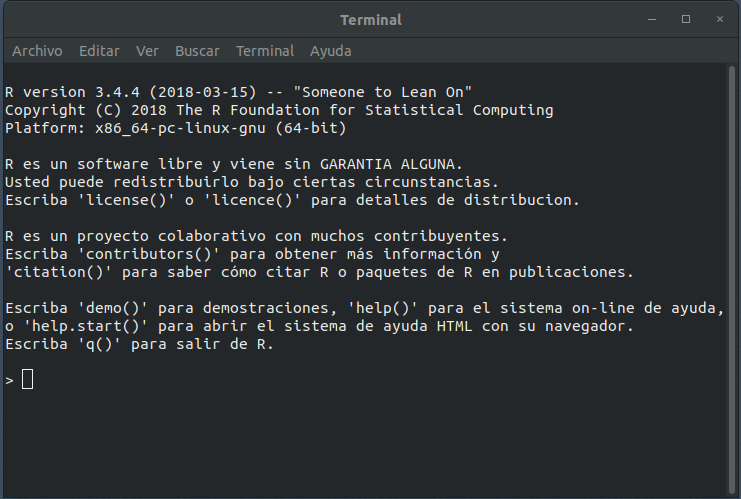
\includegraphics[width=0.5\linewidth]{images/r_propmt} 

}

\caption{R desde la terminal}\label{fig:fig2}
\end{figure}

Las versiones de R cambian una vez al año, y de 2 a 3 veces con cambios
pequeños, por eso es una buena idea que mantengas actualizada tu
versión.

\section{RStudio}\label{rstudio}

¿Qué es una IDE? IDE es el acrónimo de \emph{Integrated Development
Environment (Entorno de Desarrollo Integrado)}. Esto quiere decir que
RStudio es una aplicación que nos entrega herramientas para hacer más
fácil el desarrollo de proyectos usando R y sobre todo cuando estemos
trabajando con datos.

Para descargar e instalar Rstudio debes ir a
\url{http//www.rstudio.com/download} y seleccionar \emph{RStudio Desktop
Open Source License} (gratuita) , cuando exista una actualización
Rstudio te avisará.

Si quedó todo bien instalado, cuando abras Rstudio deberías ver algo
así:

\begin{figure}

{\centering 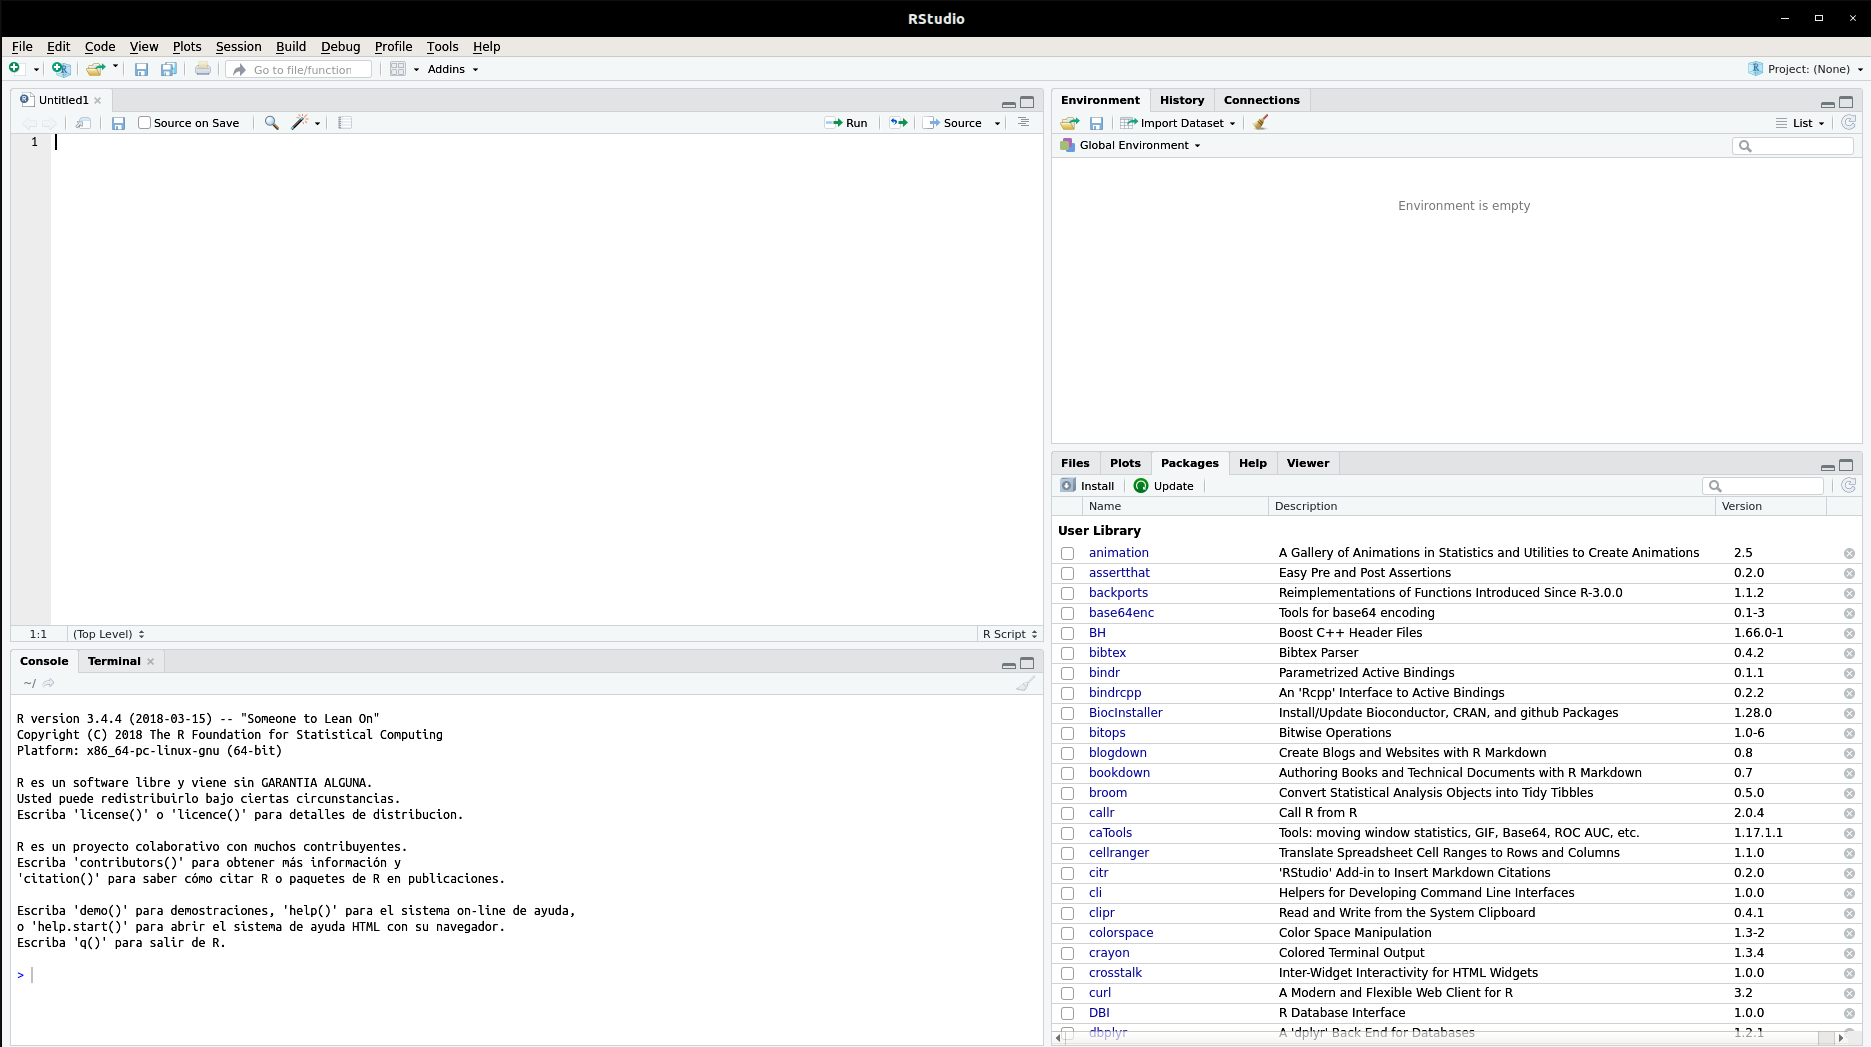
\includegraphics[width=0.5\linewidth]{images/rstudio} 

}

\caption{Rstudio}\label{fig:fig3}
\end{figure}

\begin{quote}
IMPORTANTE: Si te aparece algún error durante este proceso, lo más
probabable es que sea por alguna configuración de tu sistema operativo.
En ese caso, la mejor manera de buscar una solución es copiar el error
que arroja R, pegarlo en tu motor de búsqueda favorito y ver cómo
alguien que se enfrentó a eso antes lo resolvió.
\end{quote}

\subsection{Partes de RStudio}\label{partes-de-rstudio}

¿Para qué sirven estos paneles? Comentemos primero el panel de abajo a
la derecha. Si te fijas, el panel tiene varias ventanas:

\begin{enumerate}
\def\labelenumi{\arabic{enumi}.}
\item
  \textbf{Files} muestra el directorio (la carpeta) en la que te
  encuentras actualmente. En mi caso, no hay nada ahí porque por defecto
  RStudio me muestra el Escritorio (Desktop) y no tengo nada en él. Es
  posible que a ti te muestre otra carpeta (por ejemplo, Documentos).
\item
  \textbf{Plots} es el lugar donde aparecerán los gráficos que vayas
  creando. No hemos hecho ninguno por ahora, así que este panel también
  está vacío.
\item
  \textbf{Packages} muestra la lista de paquetes que tienes instalados
  en tu computador. Si recorres el panel verás que algunos tiene una
  marca al lado izquierdo. Eso quiere decir que el paquete está activo
  en ese momento (ya veremos cómo hacer eso). Solo los paquetes
  vinculados a R base se activan al abrir RStudio.
\item
  \textbf{Help}, como su nombre lo indica, es la pestaña en la que
  podemos encontrar ayuda. Si buscamos el nombre de un paquete o de una
  función, RStudio nos remitirá a la documentación asociada.
\item
  \textbf{Viewer} es el panel para ver contenido web generado por algún
  paquete de R (gráficos para la web o aplicaciones interactivas). Por
  el momento no lo utilizaremos.
\end{enumerate}

El panel de arriba a la derecha, por su parte, contiene el historial de
funciones que hemos ejecutado (History), la opción para generar
conexiones a bases de datos externas (Connections) y el Environment.
Este último panel es muy importante y entender lo que nos muestra es
fundamental para comprender cómo funciona R.

\section{\texorpdfstring{\emph{Scripts}}{Scripts}}\label{scripts}

El script podemos decir que es un cuarto panel\footnote{El tercer panel
  es la consola}, en donde escribiras tus códigos que queremos que
ejecute R, para crear un script debes:

\begin{enumerate}
\def\labelenumi{\arabic{enumi}.}
\tightlist
\item
  ir a
  \texttt{file\ \textgreater{}\ New\ File\ \textgreater{}\ R\ Script}
\item
  Otra forma es un atajo de teclado, \texttt{control\ +\ shift\ +\ n}
  (Linux/Windows) y \texttt{comando\ +\ shift\ +\ n} (Mac OS).
\item
  O bien ir a la barra superior de la ventana y seleccionar el tipo de
  archivo a trabajar.
\end{enumerate}

\section{Proyectos}\label{proyectos}

Una de las ventajas de RStudio es que permite crear ``proyectos''. Un
projecto es un espacio o contexto de trabajo asociado a una carpeta en
particular, en la que se guardan nuestro(s) script(s), archivos de
datos, etc. Cuando creamos un proyecto en RStudio, se crea un tipo
especial de archivo (.Rproj) que lo que hace es vincular todo lo que se
encuentra dentro de esa carpeta.

\subsection{¿Por qué esto es útil?}\label{por-que-esto-es-util}

Si parte de nuestro script, por ejemplo, implica abrir un archivo que
está en la carpeta de nuestro proyecto, no necesito indicar en mi código
toda la ruta del archivo: lo que hará RStudio será buscarlo en el
entorno/carpeta del proyecto. Si movemos la carpeta a otro lugar de
nuestro computador o la compartimos con otra persona, nuestro código
seguirá funcionando, ya que el archivo .Rproj mantendrá todo unido. Si
no creara un proyecto, tendría que indicar al inicio de mi script cuál
es la ruta de la carpeta que ocuparé como espacio de trabajo. El
problema de esa opción es que si muevo la carpeta o le cambio el nombre,
tendría que volver a escribir la ruta para que todo funcione. Al crear
un proyecto eso deja de ser una preocupación.

\subsection{¿Cómo crear un projecto?}\label{como-crear-un-projecto}

\begin{enumerate}
\def\labelenumi{\arabic{enumi}.}
\tightlist
\item
  Puedes hacerlo desde el menú File \textgreater{} New Proyect.
\item
  Lo primero que nos pregunta es si queremos crearlo en una carpeta
  nueva o en una ya existente. Elegiremos esta vez una carpeta nueva,
  así que seleccionaremos New Directory.
\item
  La siguiente pregunta es qué tipo de proyecto queremos crear. En esta
  ocasión, elegiremos la primera: \emph{New Project}.
\item
  Finalmente, le damos un nombre al proyecto y decidimos en qué parte de
  nuestro computador queremos que viva la carpeta que lo contiene.
\item
  Luego de apretar Create Project, RStudio se reinicia y se producen
  algunos cambios. El panel Files (abajo a la derecha) ahora nos muestra
  la carpeta de nuestro proyecto y el único archivo que hay en ella por
  ahora. Ese es el archivo mágico que mantiene unido todo lo que hay
  dentro de la carpeta. Cuando queramos volver a trabajar en nuestro
  proyecto, solo tenemos que abrir ese archivo.
\end{enumerate}

\begin{quote}
IMPORTANTE: RStudio ejecuta sesiones independientes de R para cada
proyecto. Es decir, si tuvieras otro proyecto abierto te aparecería otro
ícono, con su respectivo nombre. Esto nos permite trabajar en dos
proyectos en paralelo sin que se nos mezclen los objetos del entorno, el
código, los archivos, etc. Cada cosa en su lugar.
\end{quote}

\section{\texorpdfstring{\emph{Packages}}{Packages}}\label{packages}

Cuando instalamos R por primera vez en nuestro computador, lo que
estamos instalando es lo que se conoce como ``R Base'', es decir, los
elementos centrales del lenguaje de programación. Una de las ventajas de
R es que se trata de un lenguaje extensible: la propia comunidad de
usuarios puede desarrollar nuevas posibilidades para utilizarlo. La
manera de compartir estos nuevos desarrollos es a través de
``paquetes'', que incluyen, entre otras cosas, código y datos. Una
analogía que se suele utilizar para explicar esto es que R Base es un
teléfono celular tal como viene de fábrica y los paquetes las apps que
descargamos para que tenga más funcionalidades.

Para usar las librerias (``packages'') debemos usar el siguiente código:

\begin{Shaded}
\begin{Highlighting}[]
\CommentTok{# instala el package}
\KeywordTok{install.packages}\NormalTok{(}\StringTok{"acá va el package"}\NormalTok{)}

\CommentTok{# lo llama}
\KeywordTok{library}\NormalTok{(}\StringTok{"acá va el package"}\NormalTok{)}
\end{Highlighting}
\end{Shaded}

\subsection{\texorpdfstring{\emph{tidyverse}}{tidyverse}}\label{tidyverse}

\textbf{tidyverse} es un ``megapaquete'' que incluye otros paquetes en
su interior. Todos los paquetes que conforman ``el Tidyverse'' comparten
la misma visión sobre el trabajo con datos y la escritura de código.
Viene a formar parte de la nueva forma de programar en R, cuyo enfoque
es netamente en realizar Data Science. Algunas librerias relevantes son:

\begin{enumerate}
\def\labelenumi{\arabic{enumi}.}
\tightlist
\item
  ggplot2: Esta librería te permite realizar graficos avanzados.
\item
  dplyr: Su objetivo es la manipulación de datos (filtrar, seleccionar,
  generar, renombrar,etc).
\item
  magrittr: Contiene la denominada \emph{pipe} ( \%\textgreater{}\% ),
  se explicará más adelante
\item
  purrr: Para realizar iteraciones.
\item
  readr: Para cargar datos en csv, lo importante que los transforma en
  tibble.
\end{enumerate}

Para instalarlo basta escribir:

\begin{Shaded}
\begin{Highlighting}[]
\CommentTok{# instala el package}
\KeywordTok{install.packages}\NormalTok{(}\StringTok{"tidyverse"}\NormalTok{)}

\CommentTok{# lo llama}
\KeywordTok{library}\NormalTok{(}\StringTok{"tidyverse"}\NormalTok{)}
\end{Highlighting}
\end{Shaded}

Si te vas a la pestaña de \emph{Packages} verás que estan seleccionadas
aquellas librerias que se encuentran en el tidyverse.

\vspace{-27pt}

\section{Ejemplo}\label{ejemplo}

En este ejemplo vamos a trabajar con \texttt{gapminder}, un paquete que
contiene una parte de los datos de Gapminder, una base de datos que
incluye información mundial sobre población, expectativa de vida, PIB
per cápita y otros. Su autor, Hans Rosling, ha hecho varias charlas
\href{https://www.ted.com/playlists/474/the_best_hans_rosling_talks_yo}{TED}
que vale la pena mirar.

Instalamos la librería

\begin{Shaded}
\begin{Highlighting}[]
\CommentTok{# instala el package}
\KeywordTok{install.packages}\NormalTok{(}\StringTok{"gapminder"}\NormalTok{)}
\end{Highlighting}
\end{Shaded}

Cargamos tanto \texttt{gapminder} como \texttt{tidyverse}

\begin{Shaded}
\begin{Highlighting}[]
\CommentTok{# lo llama}
\KeywordTok{library}\NormalTok{(}\StringTok{"gapminder"}\NormalTok{)}
\KeywordTok{library}\NormalTok{(}\StringTok{"tidyverse"}\NormalTok{)}
\end{Highlighting}
\end{Shaded}

Calculamos el promedio de la expectativa de vida para los continentes en
el 2007:

\begin{Shaded}
\begin{Highlighting}[]
\NormalTok{world.data <-}\StringTok{ }\NormalTok{gapminder}

\NormalTok{mean.lifeExp <-}\StringTok{ }\NormalTok{world.data }\OperatorTok\StringTok{ }
\StringTok{                }\KeywordTok{filter}\NormalTok{(year }\OperatorTok{==}\StringTok{ }\DecValTok{2007}\NormalTok{) }\OperatorTok\StringTok{ }
\StringTok{                }\KeywordTok{group_by}\NormalTok{(continent) }\OperatorTok
\StringTok{                }\KeywordTok{summarize}\NormalTok{(}\KeywordTok{mean}\NormalTok{(lifeExp))}
\end{Highlighting}
\end{Shaded}

\begin{Shaded}
\begin{Highlighting}[]
\NormalTok{mean.lifeExp}
\end{Highlighting}
\end{Shaded}

Lo visualizamos
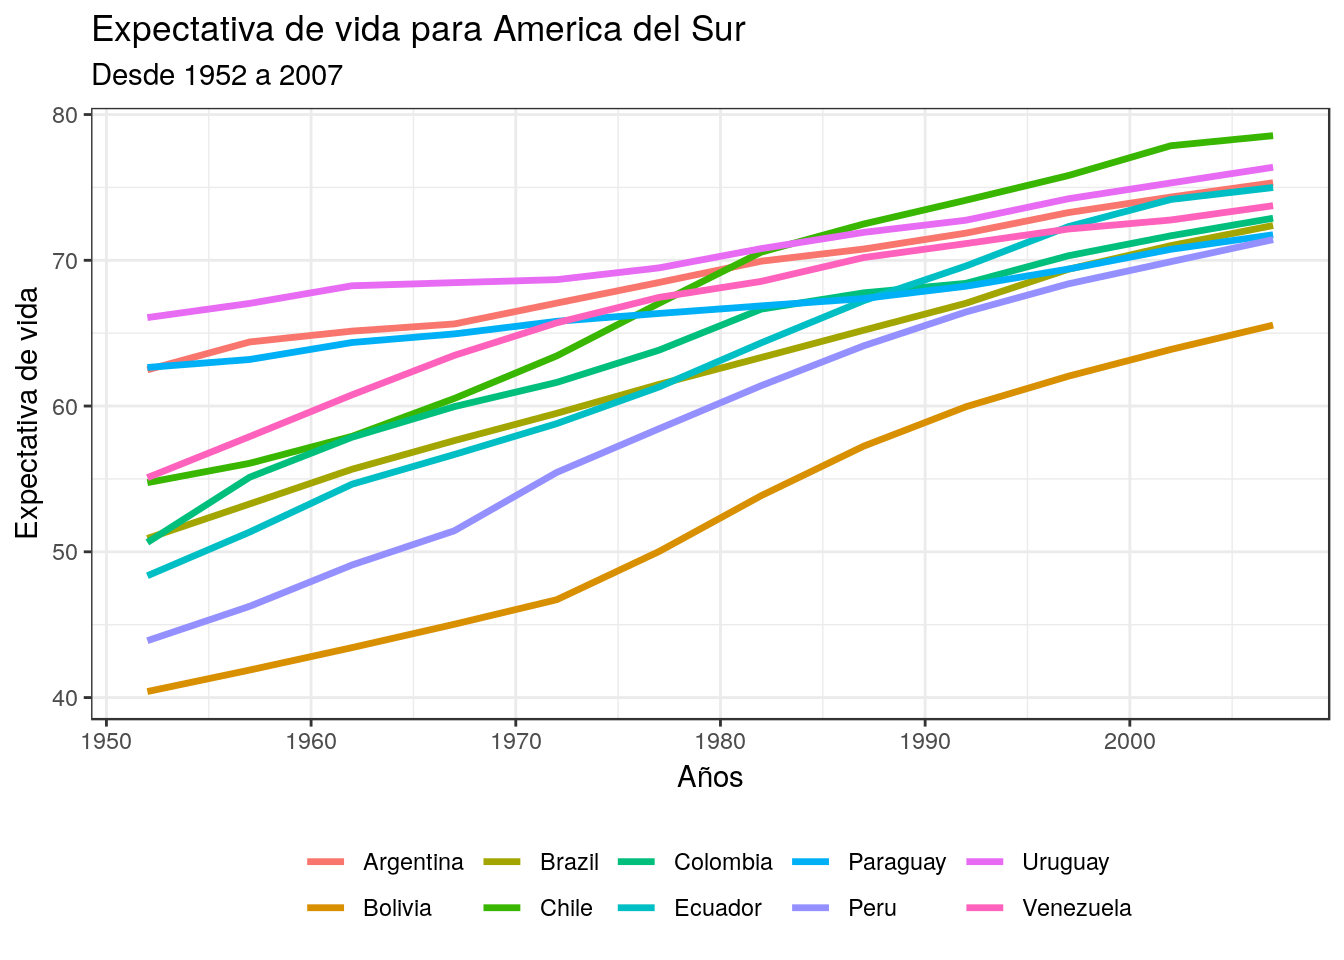
\includegraphics{bookdown-demo_files/figure-latex/unnamed-chunk-4-1.png}

Construimos la base de datos y graficamos la evolución de la expectativa
de vida para los países de America del Sur desde 1952 a 2007.

\begin{Shaded}
\begin{Highlighting}[]
\NormalTok{world.data <-}\StringTok{ }\NormalTok{world.data }\OperatorTok\StringTok{ }
\StringTok{              }\KeywordTok{filter}\NormalTok{(country }\OperatorTok\StringTok{ }\KeywordTok{c}\NormalTok{(}\StringTok{"Argentina"}\NormalTok{, }\StringTok{"Bolivia"}\NormalTok{, }\StringTok{"Brazil"}\NormalTok{, }\StringTok{"Chile"}\NormalTok{, }\StringTok{"Colombia"}\NormalTok{, }\StringTok{"Ecuador"}\NormalTok{, }\StringTok{"Paraguay"}\NormalTok{, }\StringTok{"Peru"}\NormalTok{, }\StringTok{"Uruguay"}\NormalTok{, }\StringTok{"Venezuela"}\NormalTok{))}

\NormalTok{g1 <-}\StringTok{ }\KeywordTok{ggplot}\NormalTok{(world.data) }\OperatorTok{+}\StringTok{ }\KeywordTok{geom_line}\NormalTok{(}\DataTypeTok{mapping =} \KeywordTok{aes}\NormalTok{(year,lifeExp, }\DataTypeTok{colour=}\NormalTok{ country), }\DataTypeTok{size =} \FloatTok{1.2}\NormalTok{)}
\NormalTok{g1 <-}\StringTok{ }\NormalTok{g1 }\OperatorTok{+}\StringTok{ }\KeywordTok{theme_bw}\NormalTok{() }\OperatorTok{+}\StringTok{ }\KeywordTok{labs}\NormalTok{(}\DataTypeTok{title =} \StringTok{"Expectativa de vida para America del Sur"}\NormalTok{, }\DataTypeTok{subtitle =} \StringTok{"Desde 1952 a 2007"}\NormalTok{, }\DataTypeTok{colour =} \StringTok{""}\NormalTok{) }
\NormalTok{g1 <-}\StringTok{ }\NormalTok{g1 }\OperatorTok{+}\StringTok{ }\KeywordTok{xlab}\NormalTok{(}\StringTok{"Años"}\NormalTok{) }\OperatorTok{+}\StringTok{ }\KeywordTok{ylab}\NormalTok{(}\StringTok{"Expectativa de vida"}\NormalTok{)}
\NormalTok{g1 <-}\StringTok{ }\NormalTok{g1 }\OperatorTok{+}\StringTok{ }\KeywordTok{theme}\NormalTok{(}\DataTypeTok{legend.position=}\StringTok{"bottom"}\NormalTok{) }
\NormalTok{g1}
\end{Highlighting}
\end{Shaded}

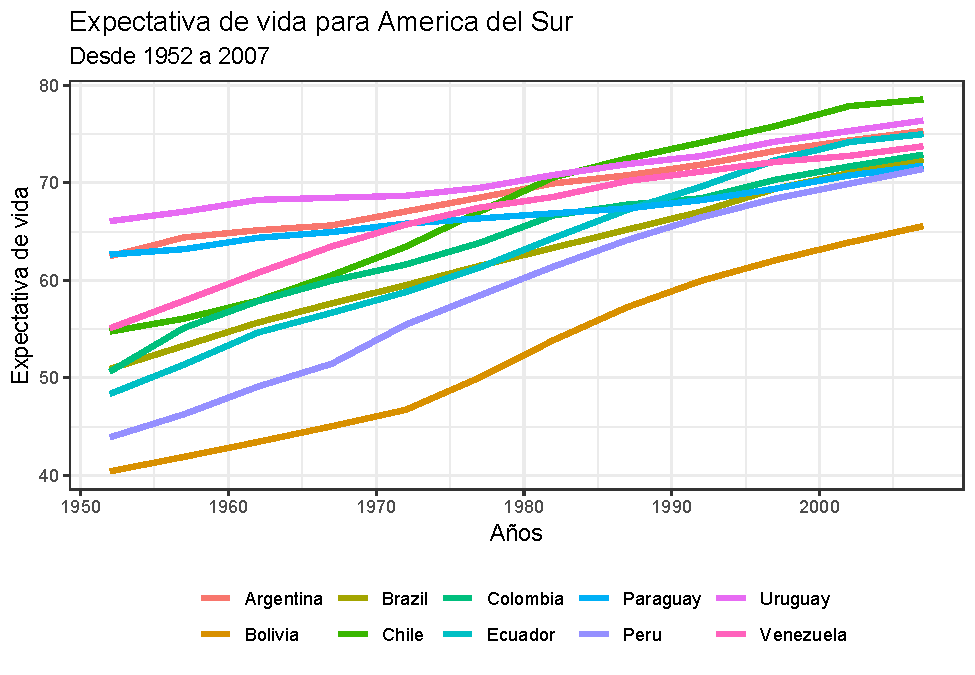
\includegraphics{bookdown-demo_files/figure-latex/unnamed-chunk-5-1.pdf}

Finalmente lo guardamos.

\begin{Shaded}
\begin{Highlighting}[]
\KeywordTok{ggsave}\NormalTok{(}\StringTok{"Grafico.png"}\NormalTok{)}
\end{Highlighting}
\end{Shaded}

\chapter{Quantmod}\label{quantmod}

\begin{quote}
IMPORTATE: Aún no está del todo listo el formato en pdf, por lo que
recomiendo verlo online.
\end{quote}

El paquete quantmod para R esta diseñado para la asistencia quantitativa
de los traders en el desarrollo de sus estrategias y modelos
financieros.

\section{¿Que es quantmod?}\label{que-es-quantmod}

Un entorno rápido, donde los operadores cuantitativos pueden explorar y
construir modelos de negociación rápida y limpiamente. A través de la
función getSymbols podemos extraer datos financieros desde varias
fuentes: Google Finance, Yahoo Finance, Federal Reserve Bank of
St.~Louis FRED (más de 11,000 series !!!) y Oanda. Incluso desde fuentes
propias: MySQL , R (Rdata) y Comma Separated Value files (csv).

No es el paquete definitivo dado que se complementa con otros, tales
como: TTR, zoo y xts. En lo que respecta al análisis técnico son las más
usadas en el mercado y usan todas las propiedades que hacen al lenguaje
R útil para realizar análisis de datos\footnote{Proximamente incluire el
  tidyquant}.

\section{Obtención de Datos}\label{obtencion-de-datos}

Para comenzar, como todo paquete en R se debe instalar

\begin{Shaded}
\begin{Highlighting}[]
\CommentTok{# Instalación package}
\KeywordTok{install.packages}\NormalTok{(}\StringTok{"quantmod"}\NormalTok{)}
\end{Highlighting}
\end{Shaded}

Una vez que esté instalado, creamos nuestro script usando
\texttt{ctrl/cmd\ +\ shift\ +\ n} y lo ``llamamos'' con

\begin{Shaded}
\begin{Highlighting}[]
\CommentTok{# Cargamos "quantmod"}
\KeywordTok{library}\NormalTok{(}\StringTok{"quantmod"}\NormalTok{)}
\end{Highlighting}
\end{Shaded}

\begin{quote}
HINT: con \texttt{ctrl\ +\ R} en windows/Linux y \texttt{cmd\ +\ R} en
MAC OS agregamos más rapido comentarios (sección) en Rstudio.
\end{quote}

\textbf{quantmod} provee una función para descargar datos desde fuentes
externas. Esta función se llama \texttt{getSymbols}, para mayor
información escribir en la linea de comandos
\texttt{?getSymbols}\footnote{No solo funcióna con \texttt{getSymbols},
  si no que con todas las funciones de distintas librerias, basta con
  ante poner \texttt{?} y luego el nombre la función}. Por defecto, se
crea un objeto en el workspace (\emph{Global Environment}) con el nombre
del ticker/nemotécnico seleccionado. Imaginemos por un momento que
necesitamos analizar el S\&P 500 desde el 2010 hasta la fecha con
periocidad diaria. Lo primero que debemos hacer es pensar desde que
fuente vamos a descargar los datos, como es un índice accionario se
recomienda usar \emph{yahoo finance}, luego buscar el nemotécnico, en
este caso es ``\^{}GSPC''.

\begin{Shaded}
\begin{Highlighting}[]
\KeywordTok{getSymbols}\NormalTok{(}\StringTok{"^GSPC"}\NormalTok{, }\DataTypeTok{src =} \StringTok{"yahoo"}\NormalTok{, }\DataTypeTok{from =} \StringTok{"2010-01-01"}\NormalTok{, }\DataTypeTok{to =} \StringTok{"2010-07-30"}\NormalTok{, }\DataTypeTok{periodicity =} \StringTok{"daily"}\NormalTok{)}
\end{Highlighting}
\end{Shaded}

\begin{verbatim}
## [1] "GSPC"
\end{verbatim}

\subsection{\texorpdfstring{¿Qué hizo la función
\texttt{getSymbols}?}{¿Qué hizo la función getSymbols?}}\label{que-hizo-la-funcion-getsymbols}

La función \texttt{getSymbols} se construye basicamente de cinco
opciones\footnote{Por el momento solo trabajaremos con estas opciones,
  exiten más.}:

\begin{enumerate}
\def\labelenumi{\arabic{enumi}.}
\tightlist
\item
  El ticker/nemotécnico, eg. \^{}GSPC.
\item
  \texttt{src}, que es la abreviación de ``source'', eg. yahoo,
  FRED\ldots{}
\item
  \texttt{from}, es el inicio de la fecha a descargar, tener presente
  que se incluye la fecha en nuestros datos.
\item
  \texttt{to}, es el final del periodo para los datos, este no se
  incluye.
\item
  \texttt{periodicity}, es la periodicidad de los datos, eg. daily,
  monthly o yearly, solo algunos datos se ajustan a las tres
  periodicidades.
\end{enumerate}

En el ejemplo anterior se descargo desde yahoo los datos del S\&P 500
desde Enero del 2010 hasta el viernes 27 de Julio del 2018 con
periodicidad diaria, construyendo un objeto en formato \textbf{xts} cuyo
nombre es GSPC.

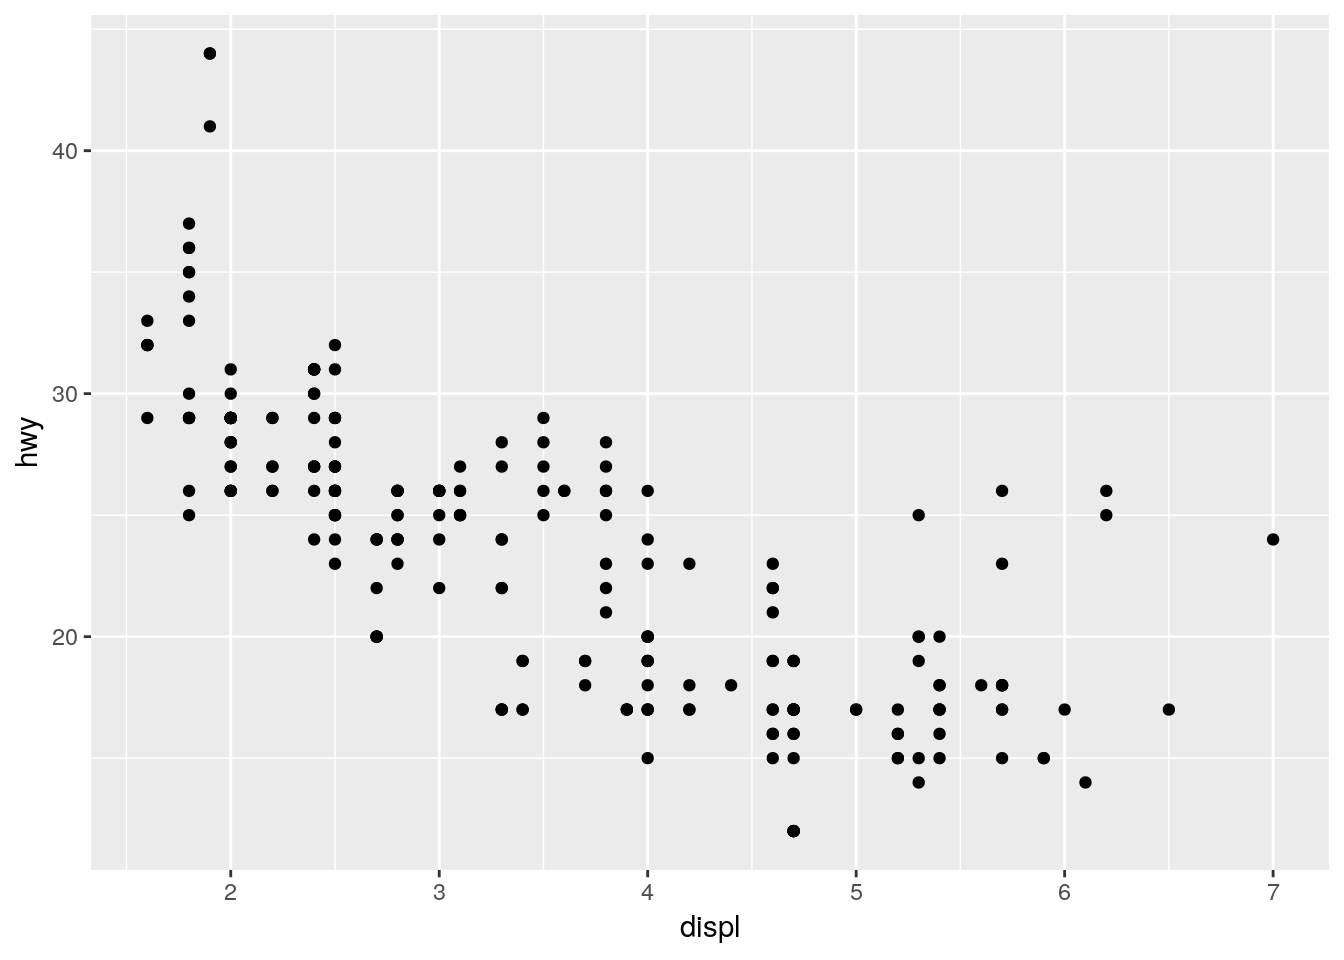
\includegraphics{bookdown-demo_files/figure-latex/unnamed-chunk-10-1.png}

\section{\texorpdfstring{Graficando con
\texttt{chartSeries}}{Graficando con chartSeries}}\label{graficando-con-chartseries}

Aún no introducimos la librería \texttt{ggplot2}, sin embargo,
\texttt{quantmod} también nos permite graficar.

\subsection{\texorpdfstring{\texttt{chartSeries}}{chartSeries}}\label{chartseries}

Para graficar basta con escribir el nombre del objeto con clase
(\texttt{class}) xts, en nuestro caso es \texttt{GSPC} que representa al
Standard and Poor 500. Si escribimos \texttt{TA\ =\ NULL},
\texttt{charSeries} no mostrará el volume\footnote{\texttt{TA} proviene
  de \emph{Technical Analysis}}

\begin{Shaded}
\begin{Highlighting}[]
\KeywordTok{chartSeries}\NormalTok{(GSPC, }\DataTypeTok{TA=}\OtherTok{NULL}\NormalTok{)}
\end{Highlighting}
\end{Shaded}

\begin{figure}

{\centering 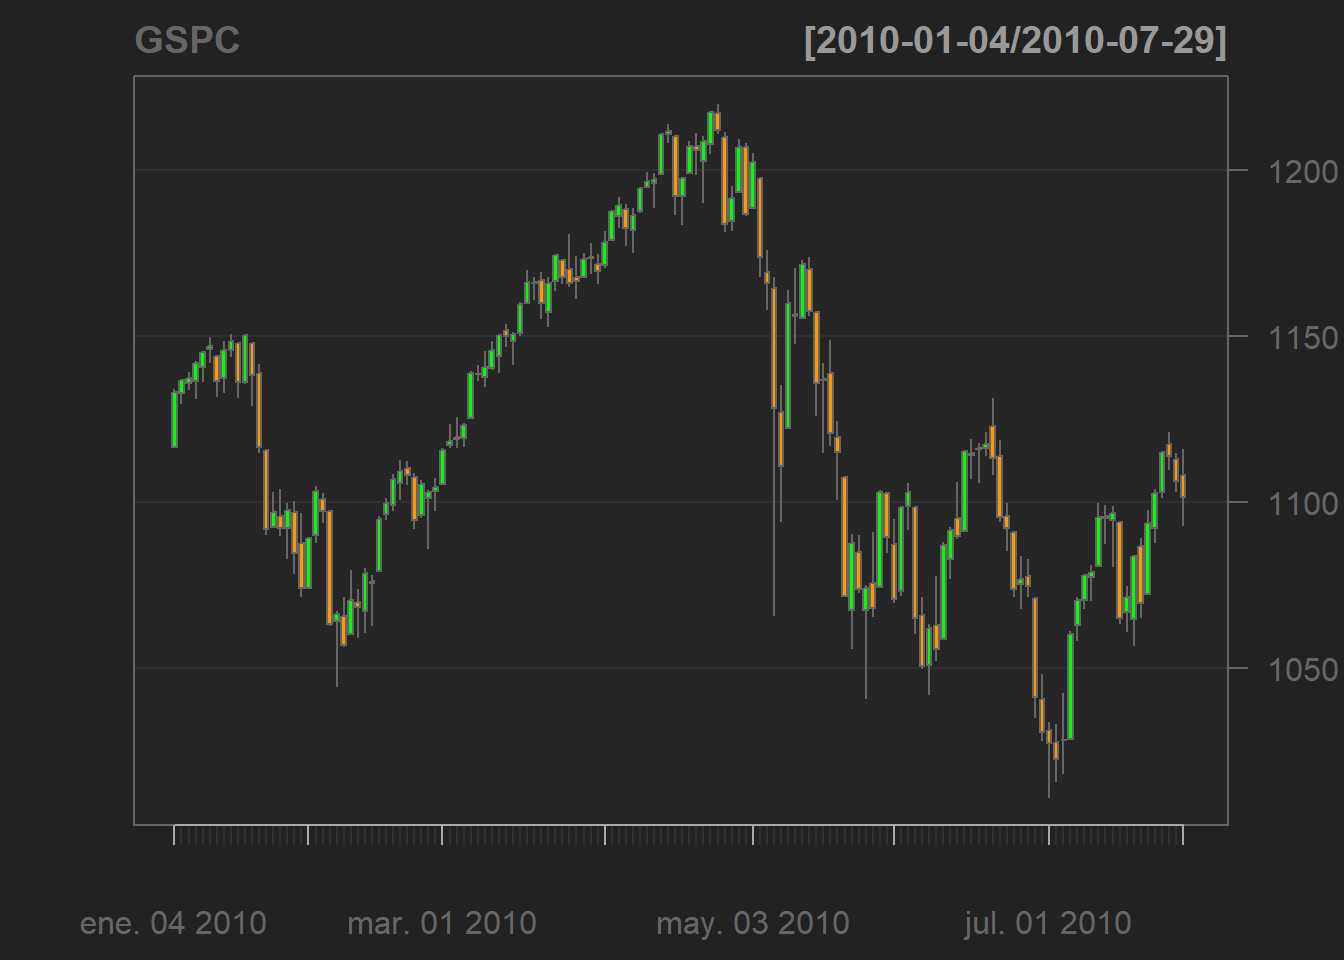
\includegraphics[width=0.75\linewidth]{bookdown-demo_files/figure-latex/unnamed-chunk-11-1} 

}

\caption{Gráfico con chartSeries con TA = NULL}\label{fig:unnamed-chunk-11}
\end{figure}

\begin{Shaded}
\begin{Highlighting}[]
\KeywordTok{chartSeries}\NormalTok{(GSPC, }\DataTypeTok{TA=}\OtherTok{NULL}\NormalTok{)}
\end{Highlighting}
\end{Shaded}

\begin{figure}

{\centering 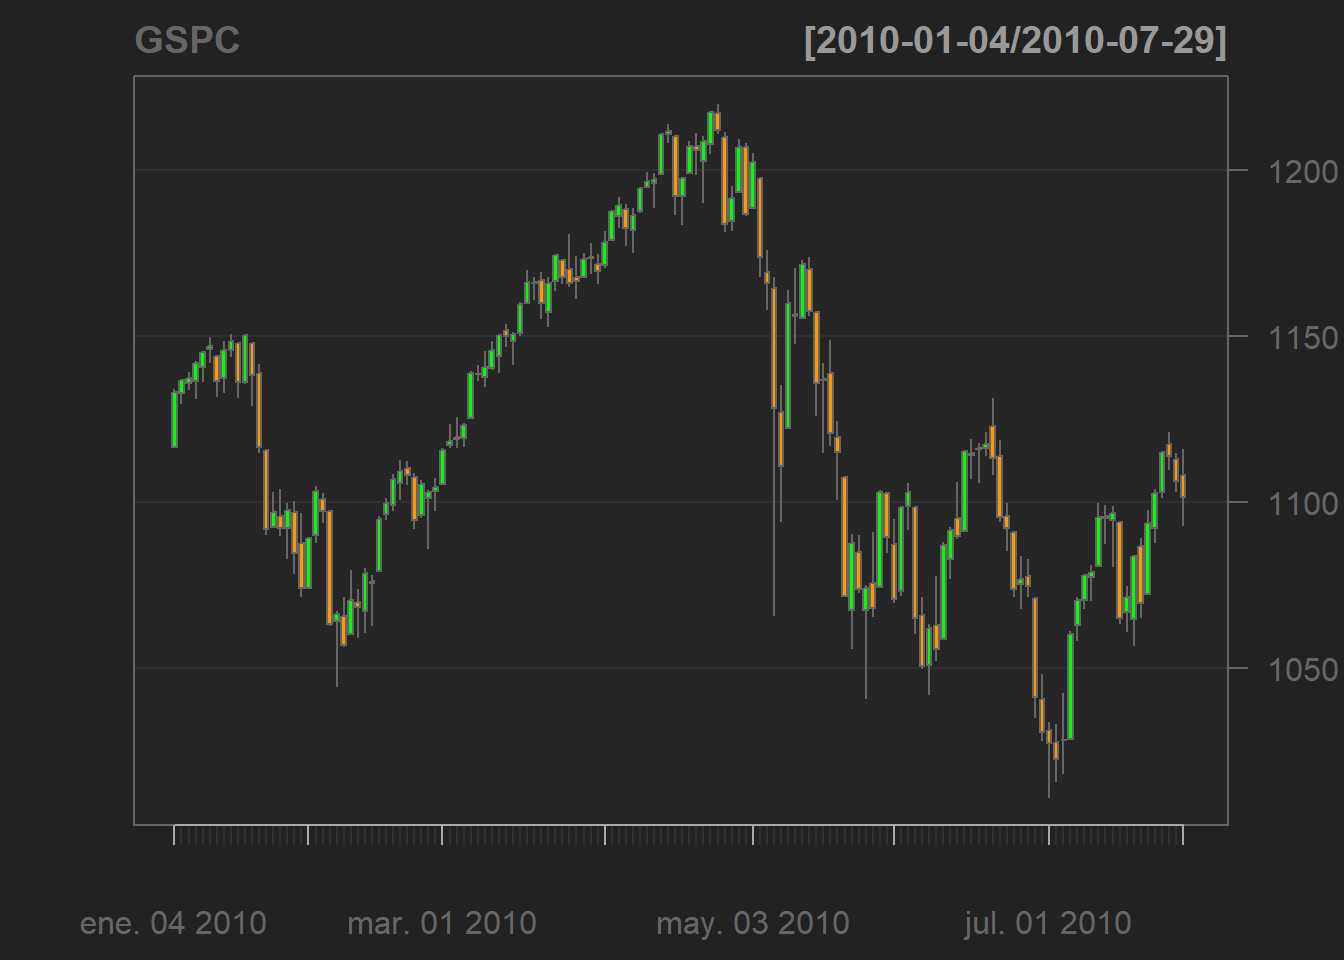
\includegraphics[width=0.75\linewidth]{bookdown-demo_files/figure-latex/unnamed-chunk-12-1} 

}

\caption{Gráfico con chartSeries sin TA = NULL}\label{fig:unnamed-chunk-12}
\end{figure}

Pero cuando las series son muy largas, podemos ver tendencias pero
dificulta ver cambios importantes a nivel de análisis técnico.

\begin{Shaded}
\begin{Highlighting}[]
\KeywordTok{chartSeries}\NormalTok{(GSPC, }\DataTypeTok{subset =} \StringTok{"last 3 months"}\NormalTok{)}
\end{Highlighting}
\end{Shaded}

\begin{figure}

{\centering 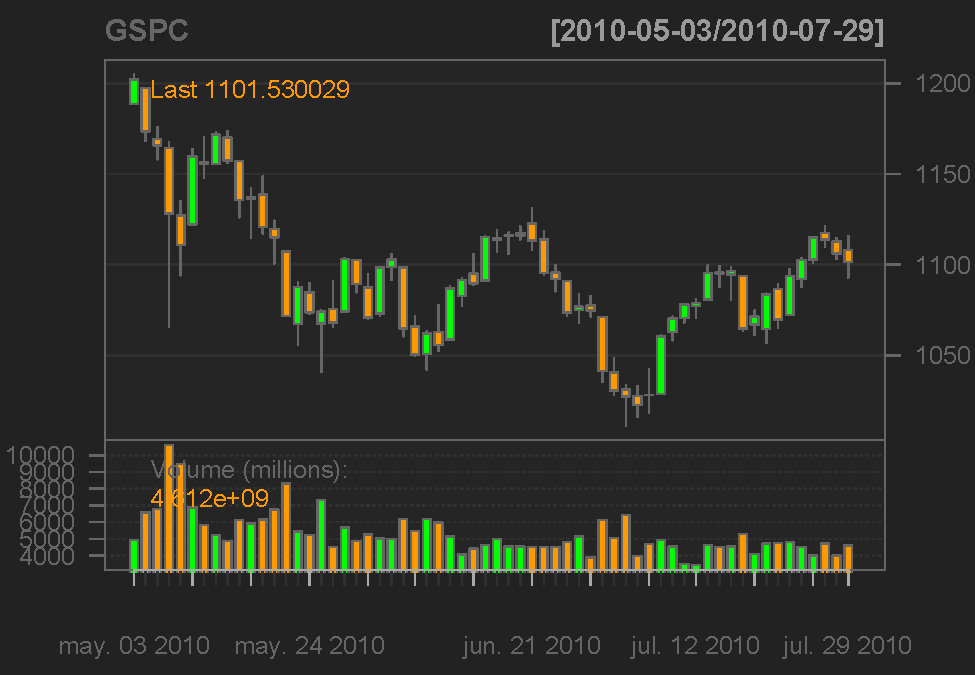
\includegraphics[width=0.75\linewidth]{bookdown-demo_files/figure-latex/unnamed-chunk-13-1} 

}

\caption{Los últimos 3 meses de GSPC}\label{fig:unnamed-chunk-13}
\end{figure}

Con el código anterior nos enfocamos solo en los tres meses anteriores.

\section{\texorpdfstring{Graficando con
\texttt{ggplot2}}{Graficando con ggplot2}}\label{graficando-con-ggplot2}

Si bien \texttt{chartSeries} es una alternativa a \texttt{plot} o
\texttt{plotly}, este no nos permite realizar gráficos que se adapten a
nuestras necesidades. ¿Qué pasa si queremos graficar retornos o retornos
acumulados? la opción por exelencia es \texttt{ggplot2}.

\subsection{\texorpdfstring{Breve introducción a
\texttt{ggplot2}}{Breve introducción a ggplot2}}\label{breve-introduccion-a-ggplot2}

Todo ggplot2 plot tiene tres componentes:

\begin{enumerate}
\def\labelenumi{\arabic{enumi}.}
\tightlist
\item
  Datos
\item
  Un conjunto de aesthetic mappings entre variables y propiedades de
  visualización.
\item
  Al menos una layer que describe la observación, son usualmente creadas
  con la función geom\_*
\end{enumerate}

\begin{Shaded}
\begin{Highlighting}[]
\KeywordTok{library}\NormalTok{(ggplot2)}
\end{Highlighting}
\end{Shaded}

A continuación usaremos la base que viene pre cargada con R cuando lo
instalamos, que es \texttt{cars}\footnote{Esta base es muy común en los
  software estadísticos y presenta datos de autos.}

\begin{Shaded}
\begin{Highlighting}[]
\KeywordTok{ggplot}\NormalTok{(mpg, }\KeywordTok{aes}\NormalTok{(}\DataTypeTok{x =}\NormalTok{ displ, }\DataTypeTok{y =}\NormalTok{ hwy)) }\OperatorTok{+}\StringTok{ }\KeywordTok{geom_point}\NormalTok{()}
\end{Highlighting}
\end{Shaded}

\begin{figure}

{\centering 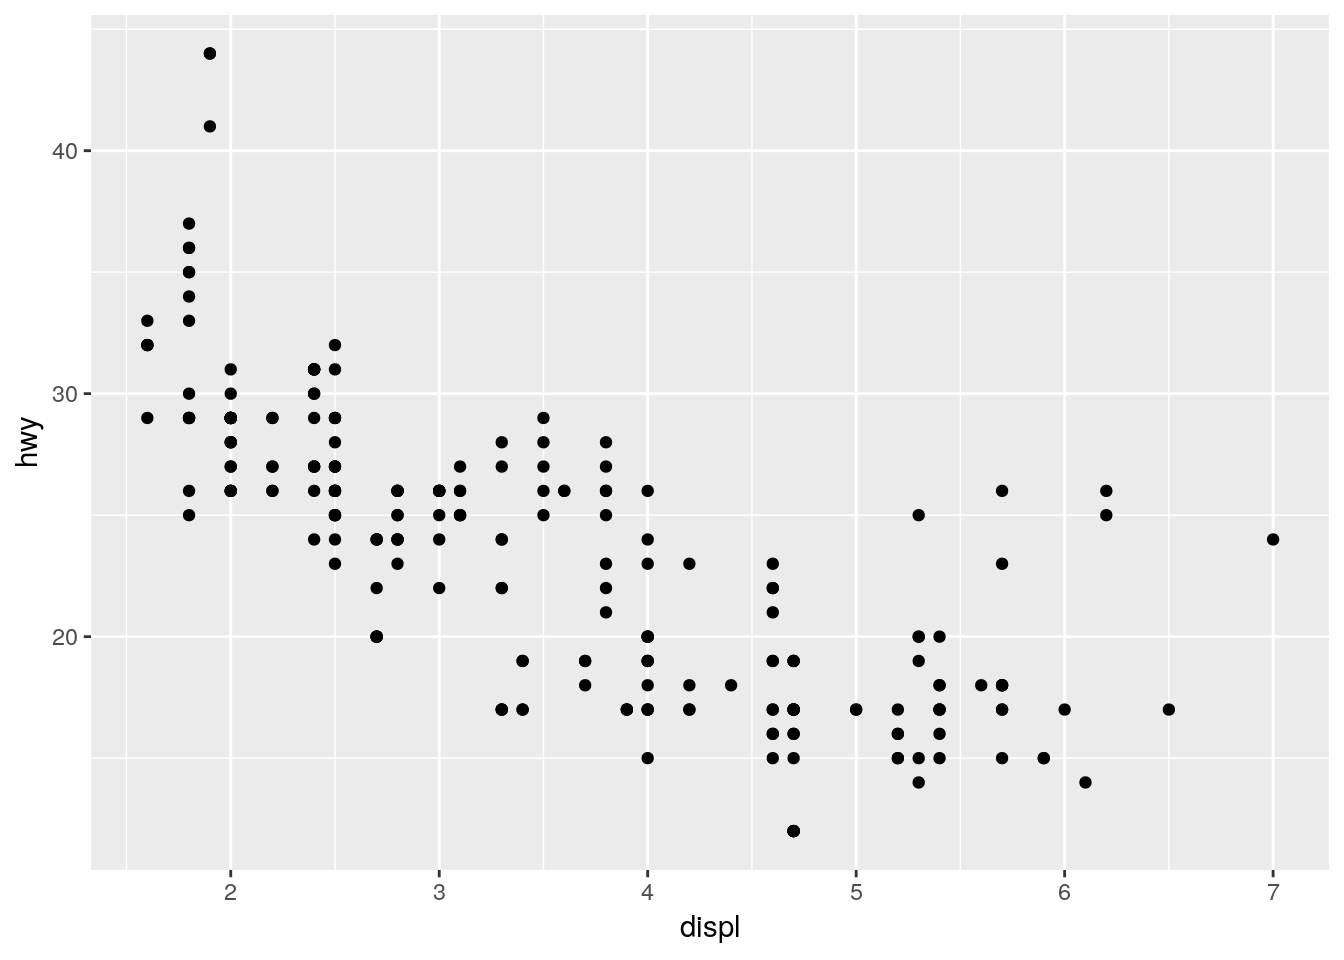
\includegraphics[width=0.75\linewidth]{bookdown-demo_files/figure-latex/unnamed-chunk-15-1} 

}

\caption{Ejemplo 1 usando ggplot2}\label{fig:unnamed-chunk-15}
\end{figure}

Esto produce el scatterplot definido como:

\begin{enumerate}
\def\labelenumi{\arabic{enumi}.}
\tightlist
\item
  Datos: mpg
\item
  Aesthetic mapping: tamaño del motor en la posición x, gasolina en la
  posición y.
\item
  Layer: puntos.
\end{enumerate}

\subsection{\texorpdfstring{Color, tamaño, forma y otros atributos del
\emph{aesthetic}}{Color, tamaño, forma y otros atributos del aesthetic}}\label{color-tamano-forma-y-otros-atributos-del-aesthetic}

Se debe usar otro aesthetics como \texttt{colour}, \texttt{shape} y
\texttt{size} (ggplot acepta los nombres americanos como británicos)

\begin{Shaded}
\begin{Highlighting}[]
\KeywordTok{ggplot}\NormalTok{(mpg, }\KeywordTok{aes}\NormalTok{(displ, cty, }\DataTypeTok{colour =}\NormalTok{ class)) }\OperatorTok{+}
\StringTok{  }\KeywordTok{geom_point}\NormalTok{() }
\end{Highlighting}
\end{Shaded}

\begin{figure}

{\centering 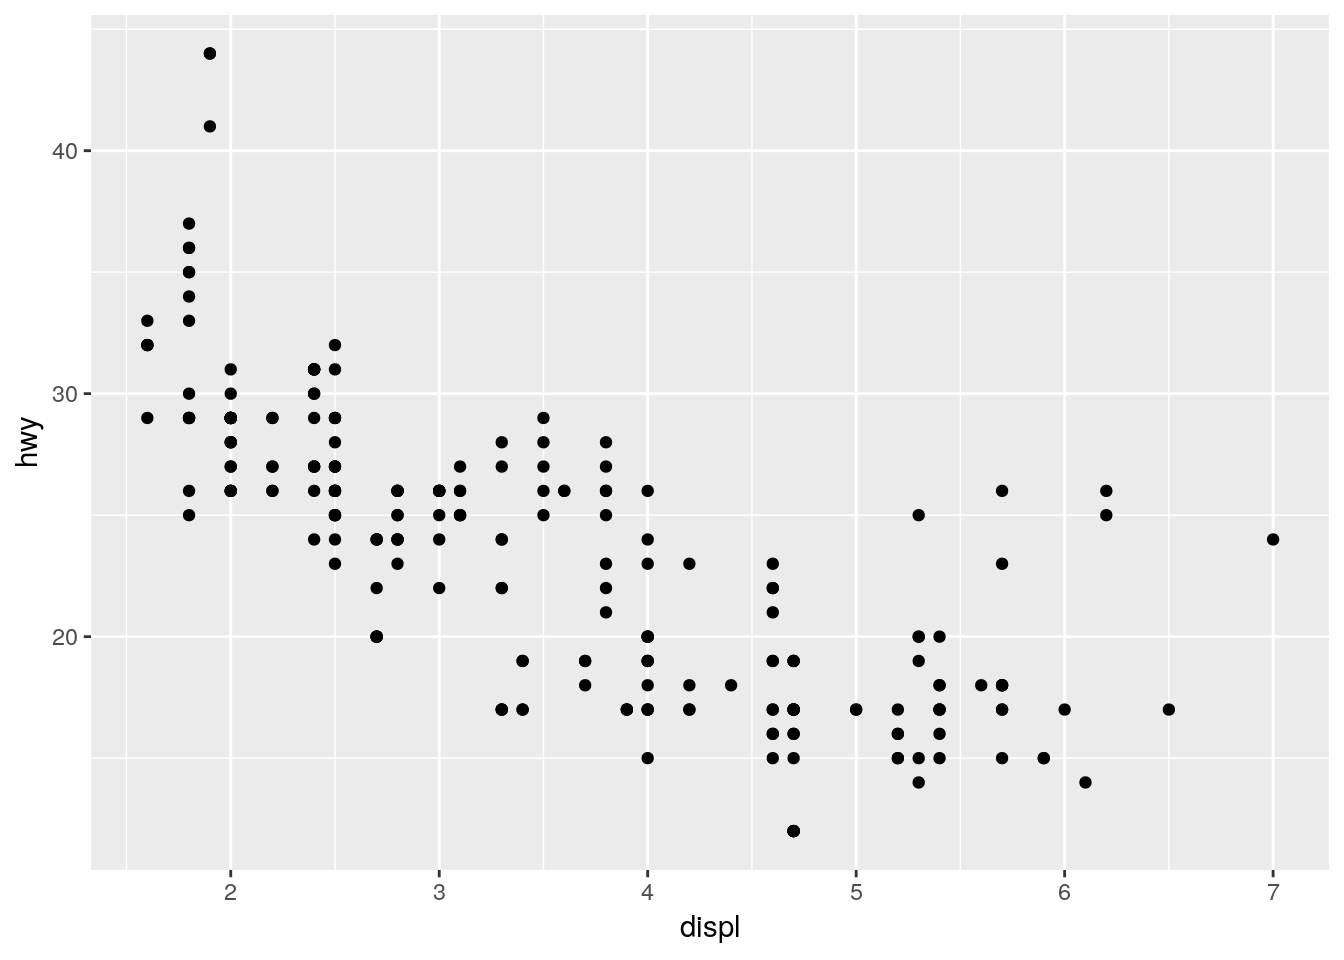
\includegraphics[width=0.75\linewidth]{bookdown-demo_files/figure-latex/unnamed-chunk-16-1} 

}

\caption{Ejemplo 2 usando ggplot2}\label{fig:unnamed-chunk-16}
\end{figure}

\begin{itemize}
\tightlist
\item
  Como se puede ver, se creo una guía con los valores, leyenda, así
  podemos ``leer'' el gráfico.
\item
  Si se quiere aesthetic para valores fijos, sin scaling:
\end{itemize}

\begin{Shaded}
\begin{Highlighting}[]
\KeywordTok{ggplot}\NormalTok{(mpg, }\KeywordTok{aes}\NormalTok{(displ, hwy)) }\OperatorTok{+}\StringTok{ }\KeywordTok{geom_point}\NormalTok{(}\KeywordTok{aes}\NormalTok{(}\DataTypeTok{colour =} \StringTok{"blue"}\NormalTok{))}
\end{Highlighting}
\end{Shaded}

\begin{figure}

{\centering 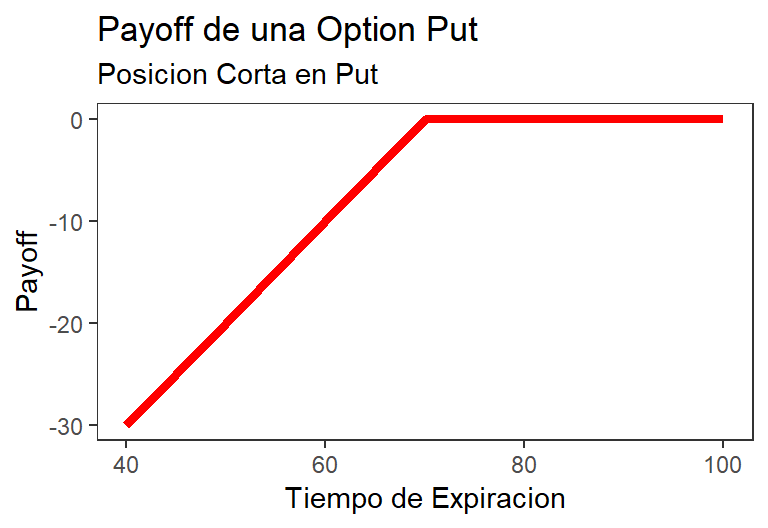
\includegraphics[width=0.75\linewidth]{bookdown-demo_files/figure-latex/unnamed-chunk-17-1} 

}

\caption{Ejemplo 3 usando ggplot2}\label{fig:unnamed-chunk-171}
\end{figure}

\begin{Shaded}
\begin{Highlighting}[]
\KeywordTok{ggplot}\NormalTok{(mpg, }\KeywordTok{aes}\NormalTok{(displ, hwy)) }\OperatorTok{+}\StringTok{ }\KeywordTok{geom_point}\NormalTok{(}\DataTypeTok{colour =} \StringTok{"blue"}\NormalTok{)}
\end{Highlighting}
\end{Shaded}

\begin{figure}

{\centering 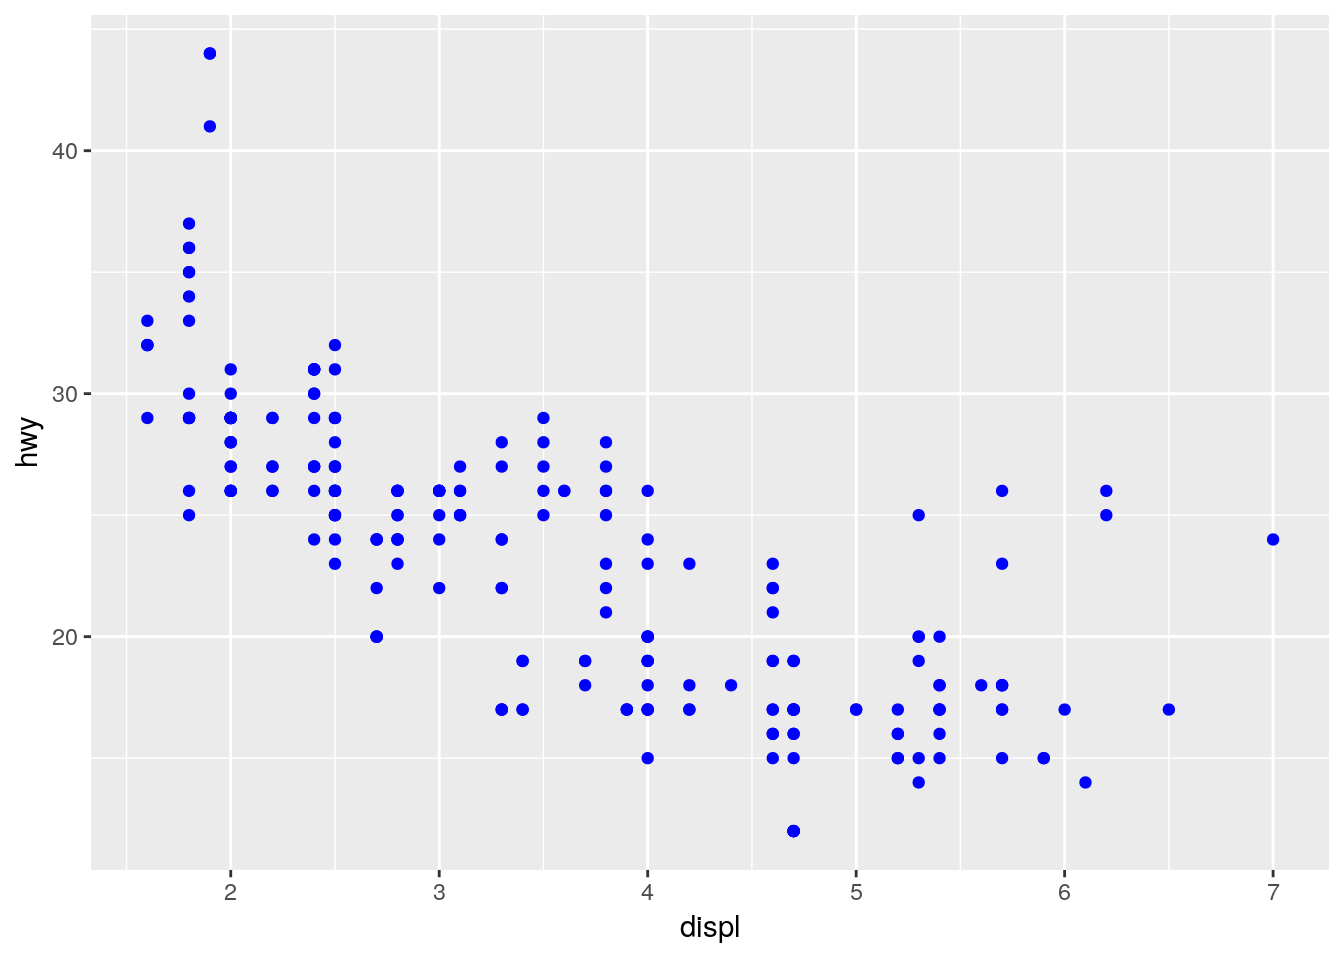
\includegraphics[width=0.75\linewidth]{bookdown-demo_files/figure-latex/unnamed-chunk-17-2} 

}

\caption{Ejemplo 3 usando ggplot2}\label{fig:unnamed-chunk-172}
\end{figure}

Ejercicios:

\begin{Shaded}
\begin{Highlighting}[]
\KeywordTok{aes}\NormalTok{(displ, hwy, }\DataTypeTok{colour =}\NormalTok{ class)}
\KeywordTok{aes}\NormalTok{(displ, hwy, }\DataTypeTok{shape =}\NormalTok{ drv)}
\KeywordTok{aes}\NormalTok{(displ, hwy, }\DataTypeTok{size =}\NormalTok{ cyl)}
\end{Highlighting}
\end{Shaded}

\begin{itemize}
\tightlist
\item
  Se recomienda usar \texttt{colour} y \texttt{shape} con variables
  categóricas.\\
\item
  Mientras que size funciona bien con variables continuas.
\end{itemize}

\subsection{\texorpdfstring{S\&P 500 con
\texttt{ggplot2}}{S\&P 500 con ggplot2}}\label{sp-500-con-ggplot2}

\begin{Shaded}
\begin{Highlighting}[]
\NormalTok{gspc <-}\StringTok{ }\KeywordTok{as.data.frame}\NormalTok{(GSPC)}
\end{Highlighting}
\end{Shaded}

\begin{Shaded}
\begin{Highlighting}[]
\NormalTok{g1 <-}\StringTok{ }\KeywordTok{ggplot}\NormalTok{(gspc) }\OperatorTok{+}\StringTok{ }\KeywordTok{geom_line}\NormalTok{(}\DataTypeTok{mapping =} \KeywordTok{aes}\NormalTok{(}\KeywordTok{index}\NormalTok{(gspc),GSPC.Adjusted))}
\NormalTok{g1 <-}\StringTok{ }\NormalTok{g1 }\OperatorTok{+}\StringTok{ }\KeywordTok{labs}\NormalTok{(}\DataTypeTok{title =} \StringTok{"S&P 500"}\NormalTok{, }\DataTypeTok{subtitle =} \StringTok{"Desde Enero 2010 a 2018"}\NormalTok{) }\OperatorTok{+}\StringTok{ }\KeywordTok{xlab}\NormalTok{(}\StringTok{"Fecha"}\NormalTok{) }\OperatorTok{+}\StringTok{ }\KeywordTok{ylab}\NormalTok{(}\StringTok{""}\NormalTok{)}
\NormalTok{g1 <-}\StringTok{ }\NormalTok{g1 }\OperatorTok{+}\StringTok{ }\KeywordTok{theme_bw}\NormalTok{()}
\NormalTok{g1}
\end{Highlighting}
\end{Shaded}

\begin{figure}

{\centering 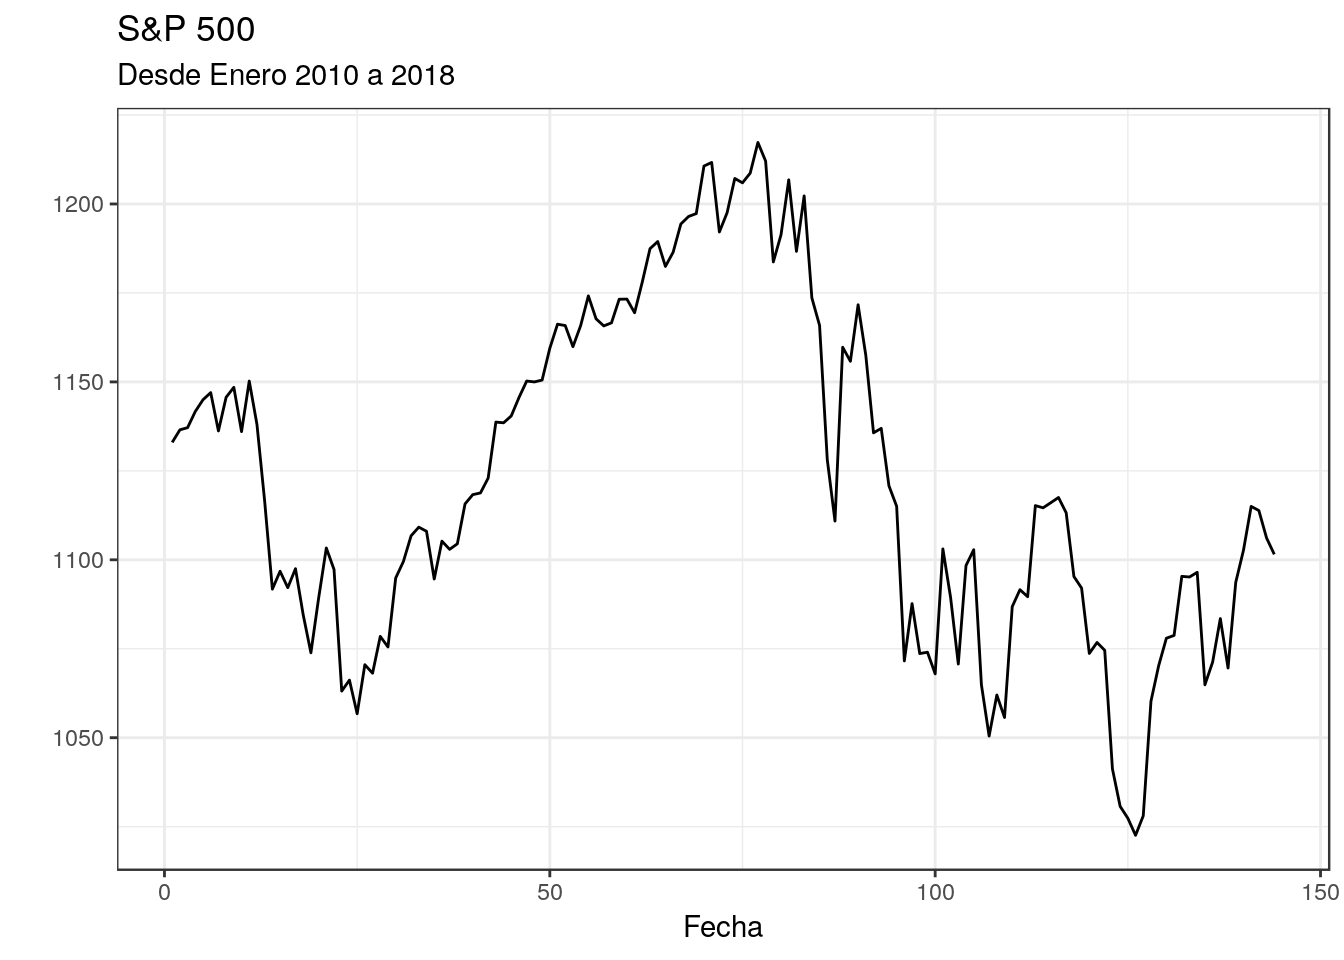
\includegraphics[width=0.75\linewidth]{bookdown-demo_files/figure-latex/unnamed-chunk-19-1} 

}

\caption{Standard and Poor 500 usando ggplot2}\label{fig:unnamed-chunk-19}
\end{figure}

\section{Multiples Datos}\label{multiples-datos}

A continuación trabajaremos con las acciones de Oracle, Nvidia, IBM y
AMD, comenzamos con crear un objeto con los nombres de los tickers

\begin{Shaded}
\begin{Highlighting}[]
\NormalTok{tickers <-}\StringTok{ }\KeywordTok{c}\NormalTok{(}\StringTok{"ORCL"}\NormalTok{,}\StringTok{"AMD"}\NormalTok{,}\StringTok{"IBM"}\NormalTok{,}\StringTok{"NVDA"}\NormalTok{)}
\end{Highlighting}
\end{Shaded}

descargamos los datos con las características requeridas, que son las
mismas que usamos anteriormente con S\&P 500

\begin{Shaded}
\begin{Highlighting}[]
\KeywordTok{getSymbols}\NormalTok{(tickers, }\DataTypeTok{src =} \StringTok{"yahoo"}\NormalTok{, }\DataTypeTok{from =} \StringTok{"2010-01-01"}\NormalTok{, }\DataTypeTok{to =} \StringTok{"2018-07-30"}\NormalTok{, }\DataTypeTok{periodicity =} \StringTok{"daily"}\NormalTok{)}
\end{Highlighting}
\end{Shaded}

\begin{verbatim}
## [1] "ORCL" "AMD"  "IBM"  "NVDA"
\end{verbatim}

Acá deben tener mucha atención:

\begin{Shaded}
\begin{Highlighting}[]
\NormalTok{list <-}\StringTok{ }\KeywordTok{lapply}\NormalTok{(tickers, }\ControlFlowTok{function}\NormalTok{(x) }\KeywordTok{Cl}\NormalTok{(}\KeywordTok{get}\NormalTok{(x)))}
\NormalTok{precio.cierre <-}\StringTok{ }\KeywordTok{do.call}\NormalTok{(merge,list)}
\end{Highlighting}
\end{Shaded}

\subsection{Retornos}\label{retornos}

La formula para calcular (log) retornos es

\[
r_t = log(1 + R_t) = log(\frac{P_t}{P_{t-1}}) = p_t - p_{t-1}
\] donde \(p_t = log(P_t)\) es llamado ``log price''.

Ahora pasamos a construir el retorno.

\begin{Shaded}
\begin{Highlighting}[]
\NormalTok{retornos <-}\StringTok{ }\KeywordTok{data.frame}\NormalTok{(}\KeywordTok{apply}\NormalTok{(precio.cierre, }\DecValTok{2}\NormalTok{, }\ControlFlowTok{function}\NormalTok{(x) }\KeywordTok{Delt}\NormalTok{(x, }\DataTypeTok{type =} \StringTok{"log"}\NormalTok{)),}
                       \DataTypeTok{fecha =} \KeywordTok{index}\NormalTok{(precio.cierre)) }\OperatorTok
\StringTok{            }\KeywordTok{rename}\NormalTok{(}\DataTypeTok{orcl =}\NormalTok{ ORCL.Close, }\DataTypeTok{amd =}\NormalTok{ AMD.Close, }\DataTypeTok{ibm =}\NormalTok{ IBM.Close, }\DataTypeTok{nvda =}\NormalTok{ NVDA.Close) }\OperatorTok\StringTok{ }
\StringTok{            }\KeywordTok{na.omit}\NormalTok{() }
\end{Highlighting}
\end{Shaded}

\subsection{Retornos Acumulados}\label{retornos-acumulados}

Si graficamos los retornos no será muy descriptivo, una forma es
trabajar con su acumulado. Con la misma lógica usamos la función
\texttt{cumsum()}.

\begin{Shaded}
\begin{Highlighting}[]
\NormalTok{acumulados <-}\StringTok{ }\KeywordTok{data.frame}\NormalTok{(}\KeywordTok{apply}\NormalTok{(retornos[}\DecValTok{1}\OperatorTok{:}\DecValTok{4}\NormalTok{], }\DecValTok{2}\NormalTok{, }\ControlFlowTok{function}\NormalTok{(x) }\KeywordTok{cumsum}\NormalTok{(x)), }\DataTypeTok{fecha =} \KeywordTok{index}\NormalTok{(precio.cierre[}\OperatorTok{-}\DecValTok{1}\NormalTok{]))}
\end{Highlighting}
\end{Shaded}

\subsubsection{Gráfico retornos
acumulados}\label{grafico-retornos-acumulados}

\begin{Shaded}
\begin{Highlighting}[]
\KeywordTok{library}\NormalTok{(}\StringTok{"reshape2"}\NormalTok{)}
\end{Highlighting}
\end{Shaded}

\begin{Shaded}
\begin{Highlighting}[]
\NormalTok{reshape <-}\StringTok{ }\KeywordTok{melt}\NormalTok{(acumulados, }\DataTypeTok{id.vars =} \StringTok{"fecha"}\NormalTok{)}
\end{Highlighting}
\end{Shaded}

\begin{Shaded}
\begin{Highlighting}[]
\NormalTok{g2 <-}\StringTok{ }\KeywordTok{ggplot}\NormalTok{(reshape) }\OperatorTok{+}\StringTok{ }\KeywordTok{geom_line}\NormalTok{(}\DataTypeTok{mapping =} \KeywordTok{aes}\NormalTok{(fecha,value, }\DataTypeTok{color =}\NormalTok{ variable))}
\NormalTok{g2 <-}\StringTok{ }\NormalTok{g2 }\OperatorTok{+}\StringTok{ }\KeywordTok{labs}\NormalTok{(}\DataTypeTok{title =} \StringTok{"Retornos Acumulados"}\NormalTok{, }\DataTypeTok{subtitle =} \StringTok{"Oracle, AMD, IBM y Nvidia"}\NormalTok{)}
\NormalTok{g2 <-}\StringTok{ }\NormalTok{g2 }\OperatorTok{+}\StringTok{ }\KeywordTok{theme_bw}\NormalTok{() }\OperatorTok{+}\StringTok{ }\KeywordTok{xlab}\NormalTok{(}\StringTok{"Fecha"}\NormalTok{) }\OperatorTok{+}\StringTok{ }\KeywordTok{ylab}\NormalTok{(}\StringTok{"Retornos Acumulados"}\NormalTok{)}
\NormalTok{g2 <-}\StringTok{ }\NormalTok{g2 }\OperatorTok{+}\StringTok{ }\KeywordTok{scale_color_manual}\NormalTok{(}\StringTok{"Tickers"}\NormalTok{, }\DataTypeTok{values =} \KeywordTok{c}\NormalTok{(}\StringTok{"red"}\NormalTok{,}\StringTok{"blue"}\NormalTok{,}\StringTok{"green"}\NormalTok{,}\StringTok{"orange"}\NormalTok{))}
\NormalTok{g2 <-}\StringTok{ }\NormalTok{g2 }\OperatorTok{+}\StringTok{ }\KeywordTok{theme}\NormalTok{(}\DataTypeTok{legend.position =} \StringTok{"bottom"}\NormalTok{)}
\NormalTok{g2}
\end{Highlighting}
\end{Shaded}

\begin{figure}

{\centering 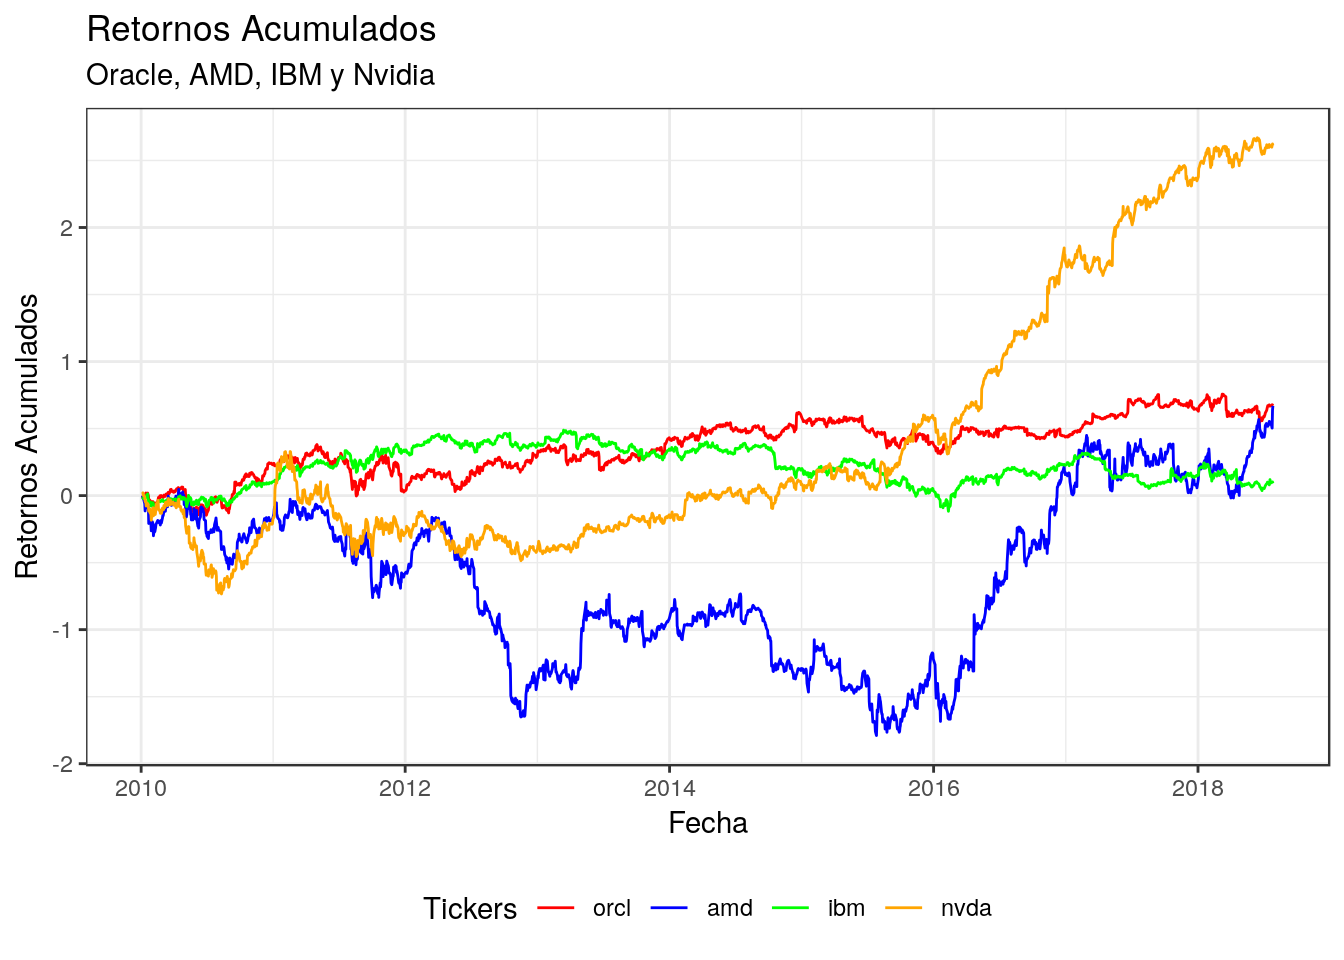
\includegraphics[width=0.75\linewidth]{bookdown-demo_files/figure-latex/unnamed-chunk-27-1} 

}

\caption{Retornos Acumulados de los tickers}\label{fig:unnamed-chunk-27}
\end{figure}

\section{Estadística Descriptiva}\label{estadistica-descriptiva}

Existe muchas formas de obtener la estadística descriptiva en R, un
librería es \texttt{fBasics}, la que a su vez contiene test de
normalidad.

\begin{Shaded}
\begin{Highlighting}[]
\KeywordTok{library}\NormalTok{(}\StringTok{"fBasics"}\NormalTok{)}
\end{Highlighting}
\end{Shaded}

\begin{Shaded}
\begin{Highlighting}[]
\NormalTok{summary <-}\StringTok{ }\KeywordTok{basicStats}\NormalTok{(retornos[}\DecValTok{1}\OperatorTok{:}\DecValTok{4}\NormalTok{])[}\KeywordTok{c}\NormalTok{(}\StringTok{"Mean"}\NormalTok{, }\StringTok{"Stdev"}\NormalTok{, }\StringTok{"Median"}\NormalTok{, }\StringTok{"Minimum"}\NormalTok{, }\StringTok{"Variance"}\NormalTok{,}
                                       \StringTok{"Maximum"}\NormalTok{, }\StringTok{"nobs"}\NormalTok{,}\StringTok{"Skewness"}\NormalTok{,}\StringTok{"Kurtosis"}\NormalTok{),]}
\end{Highlighting}
\end{Shaded}

\section{Ratio de Sharpe}\label{ratio-de-sharpe}

EL ratio de Sharpe es una medida de desempeño para portafolios, el que
se define como

\[
SR = \frac{E(R_i) - r_f}{\sigma_i}
\]

Donde \(E(R_i) = \mu_i\) es el retorno del portafolio \(i\), \(r_f\) la
tasa libre de riesgo y \(\sigma_i\) la desviaciòn estandar del
portafolio \(i\). Si asumimos como ejercicio que no diversificamos y
``construimos'' cuatro portafolios con el 100\% es invertido en cada uno
de los activos.

Para realizar el cálculo del ratio de Sharpe (SR) para Oracle

\begin{Shaded}
\begin{Highlighting}[]
\NormalTok{SR_orcl <-}\StringTok{ }\NormalTok{(}\KeywordTok{mean}\NormalTok{(retornos}\OperatorTok{$}\NormalTok{orcl) }\OperatorTok{-}\StringTok{ }\FloatTok{0.0000}\NormalTok{ )}\OperatorTok{/}\KeywordTok{sd}\NormalTok{(retornos}\OperatorTok{$}\NormalTok{orcl)}
\end{Highlighting}
\end{Shaded}

con \texttt{mean(retornos\$orcl)} vamos a obtener el promedio de la
primera columna del objeto \texttt{retornos} que es Oracle (en el
\texttt{data.frame} la columna se llama orcl, si tuviese otro nombre
como por ejemplo \texttt{perrito}, entonces hubiese sido
\texttt{mean(retornos\$perrito)}), si quisieramos AMD debería ser
\texttt{amd} y asì sucesivamente. El 0.0000 sería la tasa libre de
riesgo que la asumimos mensual y \texttt{sd(retornos{[}1{]})} nos
calcula la desviación estandar. Dado que poseemos 4 activos con sus
respectivos retornos, deberiamos construir cuatro objetos que partan con
\texttt{SR}.

\section{Test de JarqueBera}\label{test-de-jarquebera}

El test de jarque-bera usa los coeficientes de la \emph{skewness} y
\emph{kurtosis} de la muestra y se usa para testar normalidad. Otros
test comunes son el de Anderson--Darling, Cramér--von Mises, y
Kolmogorov--Smirnov.

En resumen compara que la \emph{skewness} sea 0 y la \emph{kurtosis} sea
3 bajo normalidad.

\[
JB = n{\widehat{Sk}^2 /6 + (\widehat{KUr} - 3)^2 /24}
\]

El test se encuentra en varias librerías, una de ellas es
\texttt{fBasics} que deberíamos tener instalada y cargada. Para obtener
los resultados del test para Oracle

\begin{Shaded}
\begin{Highlighting}[]
\KeywordTok{jarqueberaTest}\NormalTok{(retornos}\OperatorTok{$}\NormalTok{orcl)}
\end{Highlighting}
\end{Shaded}

Para los demàs activos hay que solo cambiar por el nombre de la columna
correspondiente.

\section{Recursos del capítulo}\label{recursos-del-capitulo}

\chapter{Introducción a teoría de portafolio}\label{portafolio}

\begin{quote}
IMPORTANTE: Aún no está del todo listo el formato en pdf, por lo que
recomiendo verlo online.
\end{quote}

\section{Librería IntroCompFinR}\label{libreria-introcompfinr}

Para la teoría de portfolio vamos a utilzar la librería IntroCompFinR
(\textbf{Intro} to \textbf{Comp}utational \textbf{Fin}ance in
\textbf{R}) creado por el profesor Eric Zivot.

\begin{enumerate}
\def\labelenumi{\arabic{enumi}.}
\tightlist
\item
  Debemos instalar primero las librerías que utiliza IntroCompFinR:
\end{enumerate}

\begin{Shaded}
\begin{Highlighting}[]
\ControlFlowTok{if}\NormalTok{(}\OperatorTok{!}\KeywordTok{require}\NormalTok{(}\StringTok{"pacman"}\NormalTok{)) }\KeywordTok{install.packages}\NormalTok{(}\StringTok{"pacman"}\NormalTok{)}
\KeywordTok{p_load}\NormalTok{(}\StringTok{"PerformanceAnalytics"}\NormalTok{,}\StringTok{"quadprog"}\NormalTok{,}\StringTok{"xts"}\NormalTok{)}
\end{Highlighting}
\end{Shaded}

\begin{enumerate}
\def\labelenumi{\arabic{enumi}.}
\setcounter{enumi}{1}
\tightlist
\item
  Ya instaladas las dependencias, descargamos IntroCompFinR :
\end{enumerate}

\begin{Shaded}
\begin{Highlighting}[]
\KeywordTok{install.packages}\NormalTok{(}\StringTok{"IntroCompFinR"}\NormalTok{, }\DataTypeTok{repos=}\StringTok{"http://R-Forge.R-project.org"}\NormalTok{)}
\end{Highlighting}
\end{Shaded}

\subsection{Funciones útiles de
IntroCompFinR}\label{funciones-utiles-de-introcompfinr}

\begin{longtable}[]{@{}ll@{}}
\toprule
\begin{minipage}[b]{0.24\columnwidth}\raggedright\strut
Funciones\strut
\end{minipage} & \begin{minipage}[b]{0.70\columnwidth}\raggedright\strut
Descripciones\strut
\end{minipage}\tabularnewline
\midrule
\endhead
\begin{minipage}[t]{0.24\columnwidth}\raggedright\strut
getPortfolio\strut
\end{minipage} & \begin{minipage}[t]{0.70\columnwidth}\raggedright\strut
Crea un portafolio (objeto)\strut
\end{minipage}\tabularnewline
\begin{minipage}[t]{0.24\columnwidth}\raggedright\strut
globalMin.portfolio\strut
\end{minipage} & \begin{minipage}[t]{0.70\columnwidth}\raggedright\strut
Computa el portafolio de mímina varianza\strut
\end{minipage}\tabularnewline
\begin{minipage}[t]{0.24\columnwidth}\raggedright\strut
efficient.portfolio\strut
\end{minipage} & \begin{minipage}[t]{0.70\columnwidth}\raggedright\strut
Computa el portafolio de mímina varianza sujeto a un retorno\strut
\end{minipage}\tabularnewline
\begin{minipage}[t]{0.24\columnwidth}\raggedright\strut
tangency.portfolio\strut
\end{minipage} & \begin{minipage}[t]{0.70\columnwidth}\raggedright\strut
Computa el portafolio tangente\strut
\end{minipage}\tabularnewline
\begin{minipage}[t]{0.24\columnwidth}\raggedright\strut
efficient.frontier\strut
\end{minipage} & \begin{minipage}[t]{0.70\columnwidth}\raggedright\strut
Computa la frontera eficiente\strut
\end{minipage}\tabularnewline
\bottomrule
\end{longtable}

\section{Cargando la librería y la base de
datos}\label{cargando-la-libreria-y-la-base-de-datos}

Una vez la instalada la librería, procedemos a cargarla en conjunto con
aquellas que utilizaremos en esta ayudantía:

\begin{Shaded}
\begin{Highlighting}[]
\ControlFlowTok{if}\NormalTok{(}\OperatorTok{!}\KeywordTok{require}\NormalTok{(}\StringTok{"pacman"}\NormalTok{)) }\KeywordTok{install.packages}\NormalTok{(}\StringTok{"pacman"}\NormalTok{)}
\KeywordTok{p_load}\NormalTok{(}\StringTok{"IntroCompFinR"}\NormalTok{,}\StringTok{"readxl"}\NormalTok{,}\StringTok{"tidyverse"}\NormalTok{)}
\end{Highlighting}
\end{Shaded}

Como ya está cargado \texttt{readxl} cargamos el archivo
\textbf{stocks.xlsx}, que ya posee los retornos\footnote{si quieren
  replicarlo vean los videos}.

\begin{Shaded}
\begin{Highlighting}[]
\CommentTok{# acá están los retornos ya calculados, para replicarlos vean el apunte}
\NormalTok{stocks <-}\StringTok{ }\KeywordTok{read_xlsx}\NormalTok{(}\StringTok{"datasets/stocks.xlsx"}\NormalTok{)}
\end{Highlighting}
\end{Shaded}

Considerando tres activos riesgosos (Starbucks, Nordstrom y Microsoft),
definimos un vector columna \(3x1\) el que tendrá los retornos y los
pesos:

\[
\mathbf{R} = 
\begin{pmatrix}
    R_{a}  \\
    R_{b}  \\
    R_{c} 
\end{pmatrix}
,
\mathbf{x} =
\begin{pmatrix}
    x_{a} \\
    x_{b} \\
    x_{c}
\end{pmatrix}
\]

El vector de retornos esperados es:

\[
E[\mathbf{R}] = E 
\begin{bmatrix} 
\begin{pmatrix}
    R_{a}  \\
    R_{b}  \\
    R_{c} 
\end{pmatrix}
\end{bmatrix}
    = 
\begin{pmatrix}
  E[R_{a}]  \\
  E[R_{b}]  \\
  E[R_{c}] 
\end{pmatrix}
    =
\begin{pmatrix}
    \mu_{a}  \\
    \mu_{b}  \\
    \mu_{c} 
\end{pmatrix}
    =
\mathbf{\mu}
\]

La matriz \(3x3\) de varianza y covarianza de los retornos es:

\[
var[\mathbf{R}] = 
\begin{pmatrix}
    \sigma^2_{a} & \sigma_{ab}  & \sigma_{ac} \\
    \sigma_{ab}  & \sigma^2_{b} & \sigma_{bc} \\
    \sigma_{ac}  & \sigma_{bc}  &  \sigma^2_{c}  
\end{pmatrix}
    =
\Sigma
\]

Notar que la matriz de covarianza es simétrica
(\(\Sigma = \Sigma^{'}\)).

Para construir las matrices anteriores en R:

\begin{Shaded}
\begin{Highlighting}[]
\CommentTok{# Promedio}
\NormalTok{mean <-}\StringTok{ }\KeywordTok{apply}\NormalTok{(stocks[}\DecValTok{2}\OperatorTok{:}\DecValTok{4}\NormalTok{], }\DecValTok{2}\NormalTok{ , }\ControlFlowTok{function}\NormalTok{(x) }\KeywordTok{mean}\NormalTok{(x)) }
\CommentTok{# Desviación Estandar}
\NormalTok{sd   <-}\StringTok{ }\KeywordTok{apply}\NormalTok{(stocks[}\DecValTok{2}\OperatorTok{:}\DecValTok{4}\NormalTok{], }\DecValTok{2}\NormalTok{ , }\ControlFlowTok{function}\NormalTok{(x) }\KeywordTok{sd}\NormalTok{(x))}
\CommentTok{# Covarianza}
\NormalTok{cov  <-}\StringTok{ }\KeywordTok{cov}\NormalTok{(stocks[}\DecValTok{2}\OperatorTok{:}\DecValTok{4}\NormalTok{])   }
\end{Highlighting}
\end{Shaded}

\bibliography{book.bib,packages.bib}

\end{document}
